\documentclass[11pt,a4paper,twoside,final]{book}
%
\usepackage{ngerman}            %Neue Rechtschreibung
\usepackage{graphicx}           %Graphiken einbinden
%\usepackage[normalsize]{subfigure} %Teilbilder in Bildern mit Querverweis
\usepackage{fontenc}            %Verwenden von \"{o} \"{a} \"{u} {\ss}
\usepackage[utf8]{inputenc}   %Verwenden von ä ö ü ß
\usepackage{fancyhdr}           %Kopf-und Fusszeilen
\usepackage{theorem}			%S�tze, Beispiele und dergleichen
\usepackage{amsmath}			%Setzen von Gleichungen und Formeln
\usepackage{amssymb}			%Mathematische Symbole
\usepackage{bibgerm}			%Deutsches Literaturverzeichnis bei Verwendung von bibtex
\usepackage{longtable}			%Lange Tabellen
\usepackage{booktabs}
\usepackage{helvet}				%Wird f�r die serifenlosen Schriften auf der Titelseite ben�tigt
\usepackage[right]{eurosym}		%Das Eurosymbol
\usepackage{pdflscape}			%Drehen einzelner Seiten ins Querformat
\usepackage{siunitx}			%Setzen von Einheiten
\usepackage{multirow}
\usepackage{caption}
\usepackage{array}
\usepackage{subcaption}
\usepackage{svg}
\usepackage{tikz}				%Ein umfangreiches Paket f�r Graphiken: Nur f�r Fans
\usepackage{algorithm}
\usepackage{algorithmic}
\usepackage{txfonts}
\usepackage{float}
\usepackage{pythonhighlight}
\usepackage{listings}
\usepackage{tikz-uml}

%\usepackage{neuralnetwork}

\usetikzlibrary{positioning}
\usetikzlibrary{calc}
\usetikzlibrary{shapes.geometric}
\usetikzlibrary{shapes.arrows}
\usetikzlibrary{decorations}
\usetikzlibrary{decorations.pathmorphing}
\usetikzlibrary{decorations.text}
\usetikzlibrary{decorations.markings}
\usetikzlibrary{backgrounds}
\usetikzlibrary{intersections}
\usetikzlibrary{matrix,chains,positioning,decorations.pathreplacing,arrows}
\graphicspath{{Bilder/}{Bilder/plots/}{Bilder/infer_images/}}

\usepackage[european]{circuitikz}	%Ein Paket zum Zeichnen von Schaltungen

\usepackage{pgfplots}				%Erstellen von Plots

\usepackage[a4paper,
			textwidth = 16.5cm,
			textheight = 25cm,
			inner = 2.5cm]{geometry}
		
		
\usepackage[pdftex,
			colorlinks,
			linkcolor = black,
			citecolor = black]{hyperref}	%Verlinkungen im pdf-Dokument


%
%	Einstellung der Kopf- und Fu�zeilen
%
\pagestyle{fancyplain}
\renewcommand{\chaptermark}[1]{\markboth{#1}{}}
 \renewcommand{\sectionmark}[1]{\markright{\thesection\ #1}}
 \lhead[\fancyplain{}{\sl\thepage}]{\fancyplain{}{\sl\rightmark}}
 \rhead[\fancyplain{}{\sl\leftmark}]{\fancyplain{}{\sl\thepage}}
 \lfoot{}
 \cfoot{}
 \rfoot{}

\setlength{\parindent}{0cm}

%--------------------------------------------------------------------
%
\renewcommand\maketitle{
\begin{titlepage}

\thispagestyle{empty}
%
\begin{tabular}[t]{lp{0.25\textwidth}r}
%

\includegraphics[width = 0.25\textwidth]{./Bilder/Logo_HSRT_TEC_RGB.png}
%
&&
\includegraphics[width = 0.4\textwidth]{./Bilder/Logo_HSRT_Schwarz.jpg}
%
\end{tabular}
%

\renewcommand{\baselinestretch}{1.2}

\vspace{2cm}

\begin{center}

\sf\huge{Hochschule Reutlingen}\\
\sf\Large{Reutlingen University}\\

\vspace{2cm}

\sf\Large{-- Studiengang Mechatronik Bachelor --}\\
%
\vspace{0.5cm}

\sf\Large{Bachelor--Thesis}

\vspace{2cm}

{\sf\huge{Entwicklung eines autonomen Systems zur Bilderkennung 
mithilfe Neuronaler Netze auf dedizierter Hardware}}\\

\end{center}

\vspace{3cm}

%
\sf{
Manuel Barkey\\
Pestalozzistraße 29\\
72762 Reutlingen\\
\ \\
Matrikelnummer : 762537

}

\vspace{2cm}

\begin{tabular}{lp{0.5cm}l}
%
Betreuer:				&&Eberhard Binder		\\
Zweitbetreuer:			&&Christian Höfert		\\
Abgabedatum:			&&TT.MM.JJJJ
%
\end{tabular}

\renewcommand{\baselinestretch}{1}
%

\vfill
%


\includegraphics[width = \textwidth]{./Bilder/Silhouette_HSRT_045K.jpg}
%
\newpage
\ 
\thispagestyle{empty}
%
\end{titlepage}}

\theoremstyle{plain}
\theorembodyfont{\itshape}\theoremheaderfont{\bf}
%
%
\newtheorem{defi}{Definition}[chapter]
\newtheorem{beisp}{Beispiel}[chapter]
\newtheorem{regel}{Regel}[chapter]
%
\newenvironment{bsp}{\begin{beisp} }{\end{beisp}}%

%\setcounter{tocdepth}{1}

\newcounter{uebung}
\setcounter{uebung}{1}

		
\title{Abschlussarbeit--Titel}

%--------------------------------------------------------------------

\begin{document}


\maketitle

\setcounter{page}{1}
\setcounter{tocdepth}{1}

\tableofcontents

\thispagestyle{empty}

\chapter{Einleitung}\label{kap:einleitung}

Im Rahmen der Bachelor Arbeit wurde ein Überwachungssystem zur Wildtiererkennung,
entwickelt, welches auf einem Raspberry Pi läuft und den Nutzer bei Erkennung
bestimmter Tiere automatisch benachrichtigt, sowie das Bild and einen Server sendet.

Die Erkennung der Tiere erfolgte mithilfe Neuronaler Netze, wodurch es möglich ist 
die Überwachung gezielt nur auf bestimmte, relevante Tiere anzuwenden und so den
Datenverkehr gering zu halten. 

Die Inferenz der Neuronalen Netze wurde dabei auf einer separaten Hardware, dem 
Neural Compute Stick 2 von Intel ausgeführt.

Des weiteren wurde eine Infrarotfähige Kamera verwendet, damit das System auch
in der Nacht einsetzbar ist.


\textbf{aus ziel der Arbeit}



Wie in der Einleitung \ref{kap:einleitung} beschrieben, soll 
ein CNN Basiertes System zur Wildtiererkennung entwickelt 
werden, das für dir Inferenz den Neural Compute Stick 2 verwendet.
Dabei sollte neben der reinen Erkennung auch eine Lokalisierung 
der erkannten Tiere im Bild stattfinden. Gängige Techniken dafür 
werden im nächsten Abschnitt erläutert.
\\
Dabei soll das Deep Learing Modell im Rahmen der gegebenen 
möglichkeiten und Limitierungen der Hardware möglichst 
genau und Robust sein, sodass es auch für die graustufen 
Bilder der Infrarot Kamera zuverlässig funktioniert.
Da eine erhöht Genauigkeit auch immer mit einer größeren
Latenz für der Inferenzzeit einhergeht war dies ein mit 
zu berücksichtigender Punkt.
\\
Neben training und evaluierung eines geeigneten Deep Learning Modells,
war die Implementierung der Anwendung, welche die Inferenz 
des Modells ausführt ein weiterer Bestandteil der Arbeit.
\\
Diese soll voll autonom auf dem Raspberry Pi laufen,
über eine mobile Netzwerk Verbindung verfügen und 
mittels eines geeigneten Kommunikations Protokolls die 
die erkannten und abgespeicherten Bilder an einen
Heim Pc senden.
Des weiteren sollte eine geeignete Kamera verwendet werden, die 
sowohl normale, als auch Infrarot Aufnahmen machen kann.

\chapter{Grundlagen}\label{kap:grundlagen}

%####################  CHAPTER 1: Grundlagen  #################

Das vorliegende Kaptitel beschreibt zunächst die Grundlagen des Machine 
Learnings, mit Neuronalen Netzen allgemein und anschließend im 
Einsatz des maschinellen Sehens.

Desweiteren wird die für die Inferenz, verwendete Hardware, 
der Neural Compute Stick 2 vorgestellt.


%------------------- SECTION: Machine Learning ------------------

\section{Machine Learning}\label{sec:ml}

Beim Machine Lerining, welches ein Teilgebiet der Computerwissenschafen
ist, geht es um die Erstellung von Algorithmen, die Zusammenhänge in großen
Datenmengen erkennen, ohne explizit darauf programmiert worden zu sein.

Eine Form davon ist das \textit{Supervised Learning}, bei dem das Programm 
neben den Input Daten auch die Zugehörigen Ausgaben erhält und daraus 
dann die Regeln für Zusammenhänge ableiten soll.
Dadurch unterscheidet sich das Vorgehen wesentlich zur klassischen Programmierung,
bei bei der die Regeln vorab definiert werden müssen.


% \vspace{0.5cm}
% \begin{figure}[htb]
%     \centering
%     \def\svgwidth{0.8\columnwidth}
%     \footnotesize
%     
\tikzset{
    decision/.style={
        diamond,
        draw,
        text width=4em,
        text badly centered,
        inner sep=-1pt,
        node distance=8em
    },
    block/.style={
        rectangle,
        draw,
        text width=6em,
        %minimum widhth=6em,
        minimum height=5em,
        text centered,
        node distance=20em
    },
    arrow/.style={
        draw,
        >=latex,
        ->
    },
    textfeld/.style={
        %draw,
        text centered,
        node distance=1.5em
    }
}


\begin{tikzpicture}

    
    \node (system) [block] {Klassisches\\Programm};
    \node (system2) [block, right of=system] {Machine Learning\\Programm};

    \node [textfeld, left=of system.162] (inputs) {Daten};
    \node [textfeld, left=of system.198] (regeln) {Regeln};
    \node [textfeld, right=of system] (output) {Ausgaben};

    \node [textfeld, left=of system2.162] (inputs2) {Daten};
    \node [textfeld, left=of system2.198] (output2) {Ausgaben};
    \node [textfeld, right=of system2] (regeln2) {Regeln};
    
    \draw[arrow] (inputs) -- (system.162);
    \draw[arrow] (regeln) -- (system.198);
    \draw[arrow] (system) -- (output);
    
    \draw[arrow] (inputs2) -- (system2.162);
    \draw[arrow] (output2) -- (system2.198);
    \draw[arrow] (system2) -- (regeln2);
    

\end{tikzpicture}

% \end{figure}
% \vspace{0.5cm}



Das ableiten der Regeln erfolgt beim Machine Learning in einem 
iterativen Prozess, welcher als Training bezeichnet wird.
Dabei werden die Zusammenhänge zwischen In- und Output Daten 
als mathematische Funktion betrachtet, welche numerisch 
angenähert wird.

Bei einem linearen Zusammenhang, handelt es sich
um eine Regression und bei einem kategorischen um 
eine Klassifizierung.


Weitere Formen neben dem \textit{Supervised Learning} sind das 
\textit{Unsupervised Learning}, bei der das Programm keine Labels 
erhällt, sondern diese durch Clustering Verfahren selber finden 
soll, oder das \textit{Reinfocement Learning}, bei dem das Programm 
mit der Umwelt interagieren soll.
\\
Diese techniken wurden in der Bachelor Arbeit nicht verwendet 
und werden daher nicht näher erläutert.

%------------------- SECTION: Neuronale Netze -------------------

\subsection{Künstliche Neuronale Netze} \label{subsec:nn}

Für komplexe Input Daten, wie beispielsweise Bilder, bei denen 
die einzelnen Pixelwerte als Inputs und der Inhalt des Bildes als 
Output dienen, werden in der Regel künstliche Neuronale Netze verwendet.
Diese sind eine Form des Machine Learings und bestehen aus einer 
vielzahl an miteinander verbundener Neuronen. Durch unterschiedlich 
starke Gewichtungen der einzelnen Verbindungen, auch Gewichte genannt, 
können für unterschiedliche Input Daten die entsprechenden Outputs 
gefunden werden.

\begin{figure}[htb]
    \centering
    \label{fig:nn}
    \def\svgwidth{0.5\columnwidth}
    \footnotesize
    \begin{neuralnetwork}[height=1]
    \newcommand{\nodetextclear}[2]{}
    \newcommand{\nodetexth}[2]{$h_#2$}
    \newcommand{\nodetextx}[2]{$x_#2$}
    \newcommand{\nodetexty}[2]{$y_#2$}
    \inputlayer[count=3, bias=false, title=Input\\layer, text=\nodetextx]
    \hiddenlayer[count=4, bias=false, title=Hidden\\layer, text=\nodetexth] \linklayers
    \outputlayer[count=2, title=Output\\layer, text=\nodetexty] \linklayers
\end{neuralnetwork}
\end{figure}


Die richtige Einstellung der Gewichte, welche zunächst zufällig initialisiert werden, 
erfolgt dabei im Trainingsprozess, welcher in \ref{fig:train} schematisch
 dargestellt ist aus folgenden drei Schritten besteht.

\begin{itemize}
    \item \textit{Forward Pass} anhand aktueller Gewichte vorhersage aus den Inputs treffen
    \item \textit{Fehlerbestimmung} Abweichung zum tatsächlichen werten berechnen
    \item \textit{Backpropagation} minimierung der Fehlerfunktion durch Anpassung der Gewichte
\end{itemize}

\begin{figure}[htb]
    \centering
    \label{fig:train}
    \def\svgwidth{0.5\columnwidth}
    
\tikzstyle{process} = [rectangle, fill=blue!20, minimum width=2.5cm, minimum height=1cm, text centered, draw=black]
\tikzstyle{arrow} = [thick,->,>=stealth]

\begin{tikzpicture}[node distance=1.6cm]

  \begin{scope}[node distance=2.5cm]
    \node (nn)      [process]                   {Neuronales Netz};
    \node (pred)      [process, below of=nn]      {Vorhersage};
    \node (loss)      [process, below of=pred]      {Fehlerfunktion};
    
  \end{scope}
  
  \begin{scope}[node distance=4cm]
    \node (opt) [process, left of=pred]      {Optimierer};
    \node (weights)  [process, left of=nn] {Gewichte};
    \node (labels)   [process, right of=pred]  {Labels};
  \end{scope}

  \node (input) at (0,1.5) {Input};

  \draw[arrow] (input) -- (nn);

  \draw[arrow] (nn) -- (pred);
  \draw[arrow] (pred) -- (loss);

  \draw[arrow] (labels) |- (loss);
  \draw[arrow] (loss) -| (opt);

  \draw[arrow] (opt) -- (weights);
  \draw[arrow] (weights) -- (nn);
  
    
\end{tikzpicture}

    \caption{Trainingsablauf NN}
\end{figure}

Durch merhfaches durchlaufen der Schritte wird die Fehlerfunktion soweit minimiert, 
sodass das Modell auch für neue Input Daten die richtigen Aussagen treffen kann.


\subsubsection{Forward Pass}
Im \textit{Forward Pass} werden die Inputs durch alle Schichten hindurch 
gereicht, um in der letzten Schicht den gewünschten Output zu liefern.
Dabei erhält jedes Neuron die mit $w_{i}$ gewichteten Ausgabewerte aller
Neuronen der vorherigen Schicht und summiert diese zusammen mit einem konstanten 
Bias Wert $b$ auf. 
Mithilfe einer Aktivierungsfunktion wird der Wert auf eienen bestimmenten Bereich 
skalliert \ref{fig:neuron}


\begin{figure}[h]
    \centering
    \label{fig:neuron}
    \begin{tikzpicture}[
    % define styles    
    init/.style={ 
         draw, 
         circle, 
         inner sep=2pt,
         font=\Huge,
         join = by -latex
    },
    squa_draw/.style={ 
        draw,
        font=\Large,
        join = by -latex
    },
    squa/.style={ 
        font=\Large,
        join = by -latex
    }
]
% Top chain x1 to w1
\begin{scope}[start chain=1]
    \node[on chain=1] at (0,1.5cm)  (x1) {$x_1$};
    \node[on chain=1,join=by o-latex] (w1) {$w_1$};
\end{scope}
% Middle chain x2 to output
\begin{scope}[start chain=2]
    \node[on chain=2] (x2) {$x_2$};
    \node[on chain=2,join=by o-latex] {$w_2$};
    \node[on chain=2,init] (sigma) {$\displaystyle\Sigma$};
    \node[on chain=2,squa_draw,label=below:{\parbox{2cm}{\centering Aktivierungs\\ Funktion}}]   {$\delta(z)$};
    \node[on chain=2,squa,label=below:Output,join=by -latex] {$y_{out}$};
\end{scope}
% Bottom chain x3 to w3
\begin{scope}[start chain=3]
    \node[on chain=3,label=below:Inputs] at (0,-1.5cm) 
    (x3) {$x_3$};
    \node[on chain=3,label=below:Gewichte,join=by o-latex]
    (w3) {$w_3$};
\end{scope}
% Bias
\node[label=above:\parbox{2cm}{\centering Bias \\ $b$}] at (sigma|-w1) (b) {};
% Arrows joining w1, w3 and b to sigma
\draw[-latex] (w1) -- (sigma);
\draw[-latex] (w3) -- (sigma);
\draw[o-latex] (b) -- (sigma);

\end{tikzpicture}

% von https://medium.com/momenton/typesetting-neural-network-diagrams-with-tex-4920b6b9fc19
    \caption{Einzelnes Perzeptron}
\end{figure}



Um den Forward Pass für eine gesmmte Schicht, besthend aus 
einer Vielzahl an Neuronen, zu berechnen, werden die Schichten 
als Vektren und die Gewichte als Mtrizen dargestellt.
\\
Die Matrixmultiplikation aus dem Vektor der vorherigen 
Schicht $x$ der Gecwichtsmatrix $W$ ergibt die Werte des Vektors 
der aktuellen Schicht,


\begin{equation}
    \label{eq:forward}
    z = W^{T}x+b
\end{equation}

welcher anschließend elementweise einer nichtlinearen Aktivierungsfunktion
$g(z)$ übergeben wird.\\
Für mittlere Schichten wird dabei oft die in \ref{eq:relu} dargestellte
\textit{ReLU} verwendet eine Funktion die negative Werte zu 0 setzt.

\begin{equation}
    \label{eq:relu}
    g(z) = max\{0,z\}
\end{equation}

Da die Ausgabe meist einen Wahrscheinlichkeites Wert zwischen 0 und 1 
Um für die Outputs einen Wahrscheinlichkeits Wert zwischen 0 und 1 
zu erhalten, wird an der Ausgabeschicht für eine binäre Klassifikation 
die Sigmoid Funktion (\ref{eq:sidmoid}) verwendet,
welche S-Förmig zwischne 0 und 1 verläuft.

\begin{equation}
    \label{eq:sidmoid}
    g(z) = \frac{1}{1 + e^{-x}}
\end{equation}


Für eine Kategorische Ausgabe mit mehr als zwei Werten wird 
die Softmax (\ref{eq:softmax}) Funktion verwendet, welche eine Wahrscheinlichkeits 
Verteilung über alle Ausgebe Neuronen generiert.

\begin{equation}
    \label{eq:softmax}
    g(z) = \frac{e^{z}}{\sum e^{x}}
\end{equation}


\subsubsection{Fehlerbestimmung}
Die Abweichung der Schätzung, welche an den Neuronen der letzen Schicht 
vorliegen, zu den tatsächlichen Werten, den Labels, wird mithilfe einer geeigneten
Fehlerfunktion bestimmt. Für die lineare Regression wird dabei z.B. 
der absolute oder quadratischen Abstand verwendet, für ein 
Klassifizierungs Modell ist jedoch eine logarithmische Fehlerberechnung 
mit der Cross Entropy Funktion, in \ref{eq:crossentropy} dargestellt effektiver.


 \begin{equation}
    \label{eq:crossentropy}
    L = \hat{y}log(y) + (1 - \hat{y})log(1 - y)
\end{equation}

Durch den Logarithmus wird der Loss um so größer, je weiter die Schätzung $y$ vom 
tatsächlichen Wert $\hat{y}$ abweicht.
%hier plot


\subsubsection{Backpropagation}

Durch Berechnung des Gradienten der Fehlerfunktion kann ermittelt 
werden in welche Richtung die Gewichte angepasst werden müssen, sodass diese sich 
im nächsten Durchgang minimiert.

Dafür wird die die Fehlerfunktion $L$ für jede Schicht partiell nach den 
Gewichten $w$ abgeleitet, was wie in gl. \ref{eq:backprop} dargestellt mithilfe der 
Kettenregel über die Aktivierungsfunktion $z$ geschieht.


\begin{equation}
    \label{eq:backprop}
    \frac{\partial L}{\partial w} = \frac{\partial L}{\partial z}\frac{\partial z}{\partial w}
\end{equation}
Mit dem ermittelten Gradienten werden dann die Gewichte nach Gleichung \ref{eq:update_wieghts} angepasst.
\begin{equation}
    \label{eq:update_wieghts}
    w  \leftarrow w - \eta \frac{\partial L}{\partial w}
\end{equation}

wobei die \textit{Lernrate} $\eta$ die Schrittweite ist, mit der die
Anpassungen vorgenommen werden.





%------------------- SUBSECTION: Validierung -------------------
\subsection{Validierung und Overfitting}\label{subsec:validation}

Um überprüfen zu können, ob und wie gut ein Modell die Zusammenhänge
in den Trainingsdaten generalisiert hat, dh auch für neue Daten
anwendbar ist,
wird der Datensatz in einen Trainings- und einen Testdatensatz aufgeteilt.

Während des Trainings wird für beide Sätze der Fehler berechnet, 
die korrektur der Gewichte mittels Backpropagation erfolgt
jedoch nur anhand der Trainingsdaten.

Entsteht eine Abweichung der beiden Fehlerfunktion wie in 
[plot overfitting] dargestellt, findet eine Überanpassung 
an die trainingsdate \textit{Overfitting} statt.

Gründe dafür sind zu wenig Trainingsdaten oder ein zu komplexes Model, 
welches sich ähnlich einer polynomialen Funktion mit hohem Grad 
an jeden datenpunkt anpassen kann, damit kein generalisierbare 
Aussage für neue Daten mehr getroffen werden kann.


\begin{figure}[htb]
    \centering
    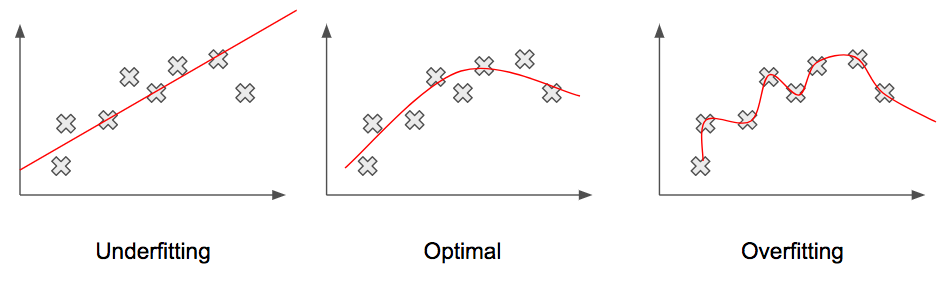
\includegraphics[width=0.8\textwidth]{over_under_fit.png}
    \caption{Quelle: \cite{deshpGuideImprovingDeep2017a}}
    \label{fig:over_under_fit}
\end{figure}

% Overfitting -> hohe varianz: varianz = train_err - test_error
% Underfitting -> hoher Bias: Bias = 

Um Overfitting, auch wenn nicht mehr Trainingsdaten 
zur Verfügung stehen zu vermeiden, gibt es verschiedene
Techniken:\\\\
\textit{Augmentierung}\\
Bei Augmentierung werden aus den vorhandenen Daten künstlich mehr 
Daten generiert, in dem an den Bildern geometrische transformationen 
oder manipulationen der pixelwerte vorgenommen werden.
\\\\
\textit{Regularisierung der Parameter (L1/L2)}\\
Bei Regularisierung wird an die Lossfuction als weiterer Term
 eine aufsummierung der Gewichte gehängt, wodurch diese bei der Minimierung 
  klein gehalten werden, wodurch weniger potential zur überanpassung da ist.
  \begin{equation}
    \label{eq:regularization}
    J(w) = E + \lambda \sum_{i} w_{i}^{2}
\end{equation}
\textit{Dropout}\\
Beim Dropout werden zufällig gewichte zu 0 gesetzt.
\\\\
\textit{Early Stopping}\\
stoppen des trainings, wenn sich overfitting einstellt.



\section{Computer Vision}

Deep Learning + Techniken der Bildverarbeitung

%---------------- SUBSECTION: Convolutional ----------------
\subsection{Convolutional Neural Networks}\label{subsec:cnn}

Convolutional Neural Networks sind eine Erweiterung 
der in \ref{sec:nn} beschriebenen Neuronalen Netze 
und besonders geeignet für die Bilderkennung.

Befor die Klassifizierung mittels Fully Connected Network 
stattfindet, sollen für die Klasse spezifische Merkmale 
aus dem Input Bild heraus extrahiert werden.

Dafür werden über das Bild zeilenweise Filtermatrizen mit kleinerer Dimension
(3x3, 5x5) geschoben und eine math Faltung angewendet.
Die Ergebnisse der Faltungen ergeben eine sog Feature Map, in welcher 
Muster die sowol in Filter Mtrix als auch in input Bild auftreten, verstärkt 
dargestellt werden.

Die Werte der Filter Matrizen entsprechen den zu lernenden Gewichten 
und werden mithilfe der Backpropagation angepasst.

\begin{figure}[htb]
    \centering
    \label{fig:conv}
    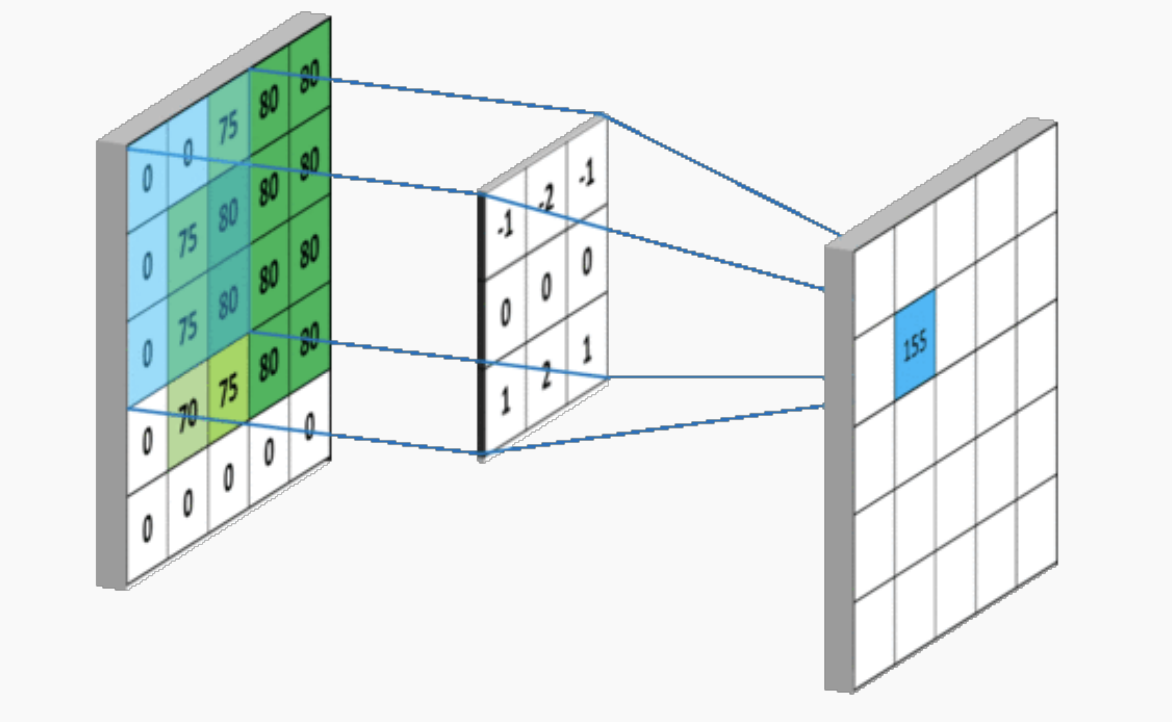
\includegraphics[width=0.4\columnwidth]{convolution.png}
    \caption{Faltung, \cite{researcherSimpleIntroductionConvolutional2019}}
\end{figure}



Durch die hintereinanderschaltung mehrerer Convolutional Layern 
lassen sich so immer komplexere Merkmale des Input Bildes in den 
Feature Maps heraus extrahieren.

Durch Subsampling Methoden wie Max Pool Layer zwischen den Convolutional
Layern verkleinert sich die Dimension der Ferture Maps in jeder Schicht.


\begin{figure}[htb]
    \centering
    \label{fig:lenet}
    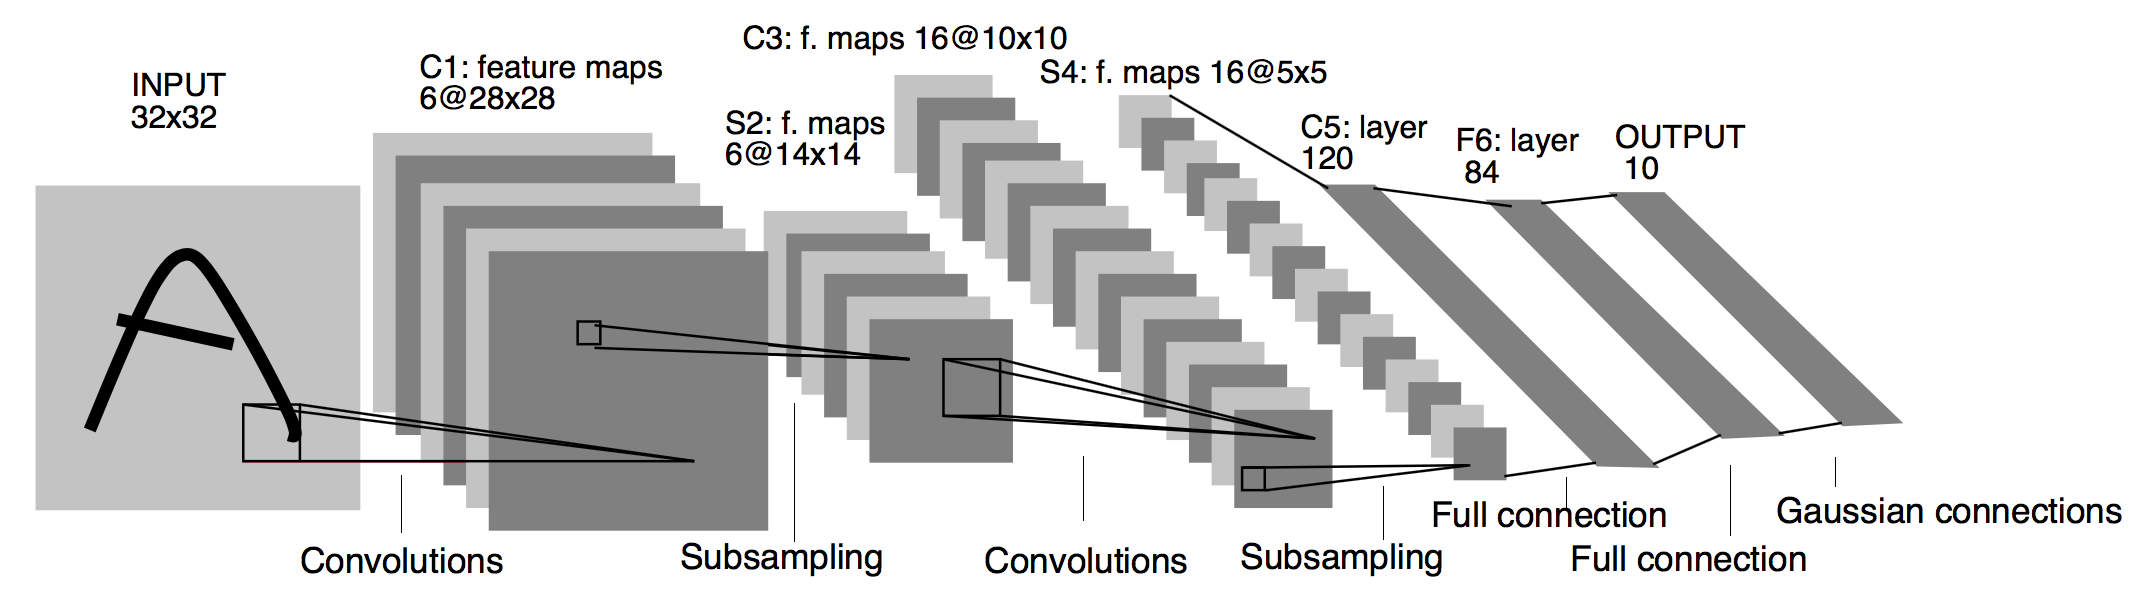
\includegraphics[width=0.8\columnwidth]{lenet.png}
    \caption{Faltung, \cite{lecunGradientBasedLearningApplied1998}}
\end{figure}


Vorteile der CNNs sind der geringere Rechenaufwand durch die gemeinsame 
Nutzung der Paramer der Filter Matrizen und die durch die 
Faltung zustande kommende räumliche invarianz für das zu erkennende 
Objekt auf dem Bild.
\\
Um die Features, welche insbesondere in den vordersten ConvLayern für 
alle klassen sehr ähnlich sind, nicht bei jedem Modell
neu lernen zu müssen, wird häufig \textit{Transfer Learing} angewendet, 
d.h. es werden die auf ein allg Datenset wie z.B. ImageNet vortrainierten
Gewichte verwendet und müssen so nur noch etwas für den eigenen Datensatz 
fine getuned werden.


\subsubsection{Architkturen}\label{subsubsec:architecture}

Nach der in Abbildung \ref{fig:lenet} dargestellten, erfolgreichen
ersten veröffentlichung eines CNN von YannLecunn 1998 \cite{lecunGradientBasedLearningApplied1998}
wurden wurden viele weitere Architekturen entwickelt. 

Diese werden anhand der ImageNet Chanllange ILSVRC \cite{ILSVRC15} bewerted

Die bekanntesten gewinner Modelle sind wie in \cite{StanfordCS231nConvolutional}
aufgeführt:


\begin{itemize}
    \item Alexnet (2012), mehrere conv layer hintereinander
    \item GoogleLeNet (2014), Inception Module
    \item VGGNet 2014
    \item ResNet (2015), 
\end{itemize}

%---------------- SUBSECTION: Obj Detection ----------------
\subsection{Objekt erkennung}\label{subsec:objdet_det}

Neben der Information, was sich auf einem Bild befindet möchte
man bei der Object Detection auch herausfinden wo sich das 
Objekt befindet.
Dafür wird ein in \ref{subsec:cnn} beschriebenes CNN als Basis 
zusammen mit weiteren Mechanaismen, auf die in \ref{sec:related_work}
genauer eingegangen wird, verwendet.
\begin{figure}[htb]
    \centering
    \label{fig:class_vs_det}
    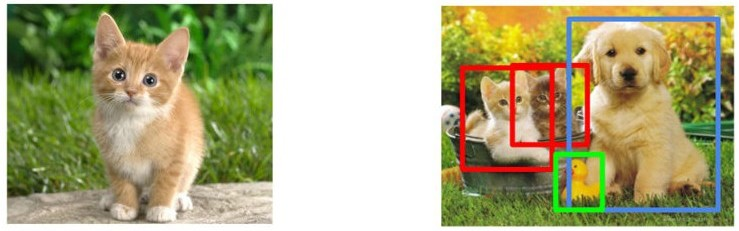
\includegraphics[width=0.8\textwidth]{classification_detection_small.jpeg}
    \caption{Unterschied: Classification - Detection}
\end{figure}


%------------------- SUBSECTION: ML Frameworks ---------------
\subsection{Deep Learing Lerining Frameworks}
\begin{itemize}
    \item Frameworks allgemein
    \item TensorFlow
\end{itemize}


%------------------- SECTION: Hardware ----------------------
\section{Inferenz}\label{sec:hardware}
%noch eine section zu Hardware allg (cpu, gpu, tpu), Neural Compute Stick und AI on the egde

\subsection{Hardware/NCS2}
Da das Training und die Inferenz von Deep Learning Algorithmen
 sehr rechenintensiv ist, werden entsprechen leistungsfähige 
Prozessoren benötigt. Dabei ist die Ausführung auf einer GPU 
(Graphical Processor Unit) meist effizienter als auf einer 
CPU (Central Processor Unit). Anwendungen auf eingebetteten Systemen
wie z.B. einplatinen Computern wie dem in der Arbeite verwendeten
Raspberry Pi kommen dabei schnell an ihre Grenzen.
Möchte man dennoch die Daten auf dem Gerät verrechnen und 
nicht an eine Cloud senden, bieten verschiedene KI Beschleuniger 
die möglichketi die Inferenz des Deep Learning Modells 
auf externer Hardware auszuführen. Einer davon ist der in der 
Arbeit verwendete Neural Compute Stick 2 von Intel.
\\
Dieser basiert auf der Movidius Myriad X Vision Processing Unit (VPU)
\cite{haussermannFunktionUndEffizienz}

\begin{figure}[htb]
    \centering
    \label{fig:ncs2}
    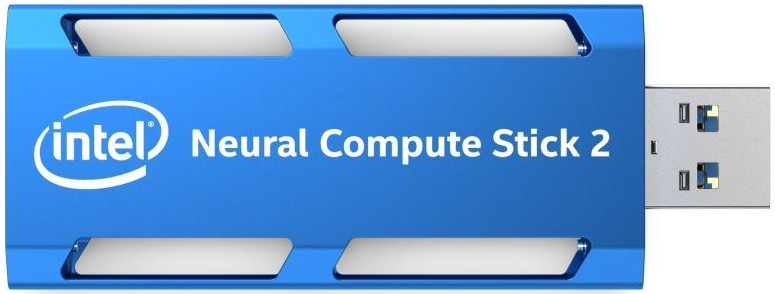
\includegraphics[width=0.4\columnwidth]{ncs2_top.jpg}
    \caption{NCS2}
\end{figure}

\subsection{Software/OpenVino}


% doku:
% https://docs.openvinotoolkit.org/latest/_docs_IE_DG_Introduction.html
% tutorial (mit guten diagrammen)
% Car
% https://github.com/intel-iot-devkit/inference-tutorials-generic/tree/openvino_toolkit_2019_r1_0/car_detection_tutorial#tutorial-step-3-add-the-second-model-vehicle-attributes-detection
% Face
% https://github.com/intel-iot-devkit/inference-tutorials-generic/blob/openvino_toolkit_2019_r1_0/face_detection_tutorial/Readme.md




Um die Inferenz eines trainierten Deep Learing Modells auf dem
Neural Compute Stick ausführen zu können, wird das Toolkit 
OpenVino verwendet.

Dieses ist eine Plattform zur Otimierung und Inferenz von 
CNN Basierten Modellen auf unterschiedlicher Intel Hardware.

Dabei wird ein eigenes Dateiformat verwendet, die \textit{Intermediate 
Representation} (IR), welche die Struktur/Architektur des Modells 
in einer .xml Datei und die trainierten Parameter/Gewichte in 
einer Binary (.bin) datei abbildet.

Mit dem \textit{Model Optimizer} können Modelle der Frameworks 
TensorFlow, Caffe, ONNX, Kaldi, oder MXNET in das IR Format 
konvertiert werden.

Um diese dann auf die entsprechende Hardware zu laden und anwendbar 
zu machen, wird die auch in OpenVino enthaltene \textit{InferenceEngeine}
verwendet.

Diese bietet eine Api mit der aus der Anwendung heraus in den 
Programmiersprachen C++ oder Python auf die Funktionen der 
InferenceEngeine zugegriffen werden können.

\begin{figure}[htb]
    \centering
    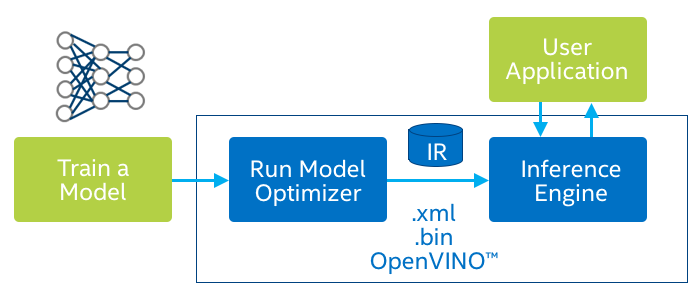
\includegraphics[width=10cm]{./Bilder/open_vino_workflow_steps.png}
    \caption{Workflow: OpenVino Toolkit}
    \label{img:openvinoworkflow}
\end{figure}

\subsubsection{InferenceEngine}

Folgendes Diagramm zeigt Aplauf und Funktionsweise der InferenceEngeine.

\begin{enumerate}
    \item HW Plugin laden
    \item Model IR einlesen
    \item In-Output Blobs allokieren 
    \item ausführbares Model laden
    \item inferenz request abgeben
    \item Bild als Array in Input Blob laden
    \item Inferenz
    \item Output verarbeiten, wieder zu Schritt 6
\end{enumerate}

\begin{figure}[htb]
    \centering
    
\tikzstyle{process} = [rectangle, minimum width=3cm, minimum height=1cm, text centered, draw=black]
\tikzstyle{arrow} = [thick,->,>=stealth]

\begin{tikzpicture}[node distance=1.6cm]
    \node (hw)      [process]                   {HW Plugin laden};
    \node (ir)      [process, below of=hw]      {Model IR einlesen};
    \node (io)      [process, below of=ir]      {In-Output Blobs};
    \node (execNet) [process, below of=io]      {executable Model};
    \node (prepIn)  [process, below of=execNet] {preprocess Input};
    \node (infer)   [process, below of=prepIn]  {infer};
    \node (procOut) [process, below of=infer]   {process Output};

    \draw [arrow] (hw) -- (ir);
    \draw [arrow] (ir) -- (io);
    \draw [arrow] (io) -- (execNet);
    \draw [arrow] (execNet) -- (prepIn);
    \draw [arrow] (prepIn) -- (infer);
    \draw [arrow] (infer) -- (procOut);
    \draw [arrow] (procOut) -- (prepIn);
    
\end{tikzpicture}

    \caption{}
    \label{}
\end{figure}



\begin{python}
    # 1.
    plugin = IEPlugin(device='MYRIAD')

    # 2.
    {\_}
    %net = IENetwork(model=model\textunderscore xml, weights=model\textunderscore bin)

%     # 3. 
%     input_blob  = net.inputs
%     output_blob = net.outputs

%     # 4.
%     exec_net = plugin.load_network(net, n_requests)

%     # 5 (ab hier loop)
%     image = preprocess(capture) 
%     # capture dims zu input blob dims transformieren
%     # img_h, img_w, img_c -> blob_n, blob_c, blob_h, blob_w

%     # 6. 
%     res = exec_net.infer({input_blob : image})

%     # 7.
%     res = res[output_blob] # enthällt zb rois

\end{python}


Output Format variert je nach Modell, Image Classification,
ObjectDetection sowie Instance Segmentation.


Um die Ausführungzeit der Inferenz zu verringern, können, 
je nach Hardware Optimierungen wie Asynchtone Inferenz, 
Inferenz requests auf mehreren Threads, oder Batching des 
Inputs vorgenommen werden.

\begin{figure}[htb]
    \centering
    \def\svgwidth{0.7\textwidth}
    \input{Bilder/synch_asynch.pdf_tex}
    \caption{Asynchron und mehrerere Inferenz Requests}
    \label{fig:async}
\end{figure}

In Abbildung \ref{fig:async} dargestellt die Asynchrone ausführung 
zwischen dem aufbereiten der Frames und der Inferenz, sowie 
mehrere parallel ausgeführte Inferenz Requests.


\chapter{Realisierung Objekt Erkennung}\label{kap:objerk}

\section{Dataset}\label{sec:dataset}


Da es sich um supervised Learning handelt müssen trainigs daten gelabelt werden.\\
für validierung und test muss datensatz zu 80, 10, 10 in test/train/validation aufgeteilt werden.
\\
wie in \ref{sec:ml} beschieben dient das validierungs set zur überwachung wärend des trainings für overfitting.\\
Mit dem Test set kann nach dem training die Inferenz also das ausfüren des traininierten models getestet werden.

Für die Objekterkennung muss der Datensatz wie in \ref{sec:deepl_cv} beschrieben neben den gelabelten bildern auch
die X- und Y-Koordinaten der Bounding Boxen, welche das objekt auf dem Bild umramt, enthalte. das Objekt befindet enthalten.\\


\subsection{Datenbeschaffung}\label{subsec:get_data}

Da das Erstellen eines eingangs erwähnten Datensets von Hand sehr müsam ist wird meistens auf Quellen zurückgegriffen, die
schon gelabelte Daten zu bestimmten Klassen zur verfügung stellen. Neben den in \ref{subsec:comp} vorgestellten Seiten
bietet OpenImages einen vielzahl an Klassen an, darunter auch Unter der Kategorie Säugetiere eine Auswahl an Wild Tier, welche 
im folgenden verwendet wurde.

Mit einem Open source Tool \cite{OpenImages} konnten eine teilmenge aus dem gesammten Open Images datensatzes herunter geladen werden.

Die Label Files haben das anotierungs format \texttt{class,xmin,ymin,xmax,ymax} welches wie in \ref{subsec:tfrecord} 
beschrieben wird, noch in ein für tensorflow vertändliches format gebracht werden musste.

Die Verteilung der Klassen im Datensatz war nicht ausbalanciert, wie in \ref{fid:distribution} zu sehen ist.

Das kann zur folge haben das.\\

Allg wie viele samples sollte man haben.\\

Augmentierung im folgenen Teil beschieben.



\subsection{Augmentierung}




was ist Augmentierung\\
wie wurde es angewand\\
bsp bilder



\subsection{TF Record Files}\label{subsec:tfrecord}

was es ist\\
wie es erstellu wurde\\

Wie in \ref{subsec:get_data} erwähnt verwendet tensorflow ein bestimmtes format für das datenset, sog 
Protocol buffer tf record files, dateien im Binary format die sowohl die Bilder als 
auch die Labels enthalten. das sind Protocol buffer welche die daten serealisieren.\\
evtl hier besp ausschnitt von aufbau eines proto elements.\\

Um nun die von OpenImages herunter geladenen Bilder und Label Files in das TFRecords Format zu bringen waren 
mehrere Schritte nötig.

OI - VOC - csv - tf.records



\section{Training}

\subsection{TF obj det api}

Für das Training wurde das Framework Tensorflow verwendet, welces eine Api für Objekterkennung bietet. 

welche pretrained modell gibt es und welche kamen in frage (für ncs2)
Die Tensorflow Objekt Detection Api bietet eine vielzahle an vortrainierten Modellen, 
dabei wurden die meiseten auf den COCO datensatz trainiert.\\

speed/acc trade off \\%\cite{paper speed/acc}

daneben war bei der bei der Ausahl die kompatibilität zu Open Vino zu berücksichtigen:\\
liste von kompatiblen modellen.\\

trainiert wurde auf:\\
\begin{itemize}
    \item ssd mobile net und inception
    \item faster rcnn (inception und resnet)
    \item frcnn
\end{itemize}

(in eval ergebniss dann etwa so: ssd zu schlechte 
performence und für appl keine realtime nitwendig, 
frcnn zu langsam, faster rcnn gute mitte)

hier ersten durchlauf (mit Overfitting) darstellen

\subsection{Regularisierung}

Um das Overfitting zu vermeiden gibt es wie in \ref{sec:nn} 
beschrieben vershiedene Möglichkeiten.

Untersucht wurde hier

\begin{itemize}
    \item Augmentierung
    \item Early Stopping
    \item \dots weitere zB $L_{1}$, $L_{2}$
\end{itemize}



\subsection{Training grayscale}\label{subsec:train_gray}

Da die Kamera im Infrarot Modus ein Graustufen Bild mit nur einem 
Farbchannel liefert, muss dies für die Inferenz berücksichtigt werden.

Es ergeben sich hier mehrere möglichkeiten:

\begin{enumerate}
    \item Normales (r, g, b) Netz
    \item Ein Farbchannel (gr) Netz
    \item Drei Farbchannel (gr, gr, gr)
\end{enumerate}

Für 1. und 3. Müssen die bilder der Kamera vor der 
Inferenz auf 3 Farbchannel ($3 \times grau$) erweitert werden.
\\
Um das Netz auf einen Channel zu trainieren wurde im config file \dots
\\
Um $3 \times gray$ zu trainieren wurden die Bilder in OpenCV in 
grau convertiert und wieder als jpgs abgespeichert.

Die Ergebnisse sind in Kapitel \ref{kap:eval} dargestellt.


\section{Parameter Optimierung}
einstellungen im Config File\\
tensorflow graph oder plot zeigen\\
loss erklären (mit formel und für train und eval)



\chapter{Evaluierung}\label{kap:eval}

In diesem Kapitel wird die Auswertung der 
Ergebnisse der trainierten Modelle beschrieben.

Dafür werden im ersten Abschnitt zunächst die Metriken 
erklärt, anhand denen die Evaluierung erfolgte. 

Im zweiten Abschnitt werden die beiden verwendeten Object detection 
Modelle \textit{SSD} und \textit{Faster R-CNN}, hinsichtlich dieser
Metriken, sowie anhand von Inferenzergebnissen verglichen.

Der dritte Abschnitt beschreibt Methoden, mit denen 
die Ergebnisse des Faster R-CNN optimiert werden konnten.

Im vierten Abschnitt werden die Modelle dann noch hinsichtlich 
der Inferenzzeit miteinander verglichen.


\section{Evaluierungs Metriken}\label{sec:metricen}

%\subsection*{Mean Average Precision (mAP)}

Zur Messung der Genauigkeit der Object detection Modelle, 
wurde die \textit{Mean Average Precision (mAP)} verwendet.
Diese bezieht sowohl Klassifikations-, als auch
Lokalisierungs Genauigkeit mit ein und
lässt sich aus den folgenden Werten berechnen.

\begin{itemize}
  \item \textit{True Positive (TP)}:
  Das Model hat richtig das Vorhandensein eines Objekts geschätzt
  \item \textit{True Negative (TN)}:
  Das Model hat richtig die Abwesenheit eines Objekts geschätzt
  \item \textit{False Positive (FP)}:
  Das Model hat fälschlicherweise das Vorhandensein eines Objekts
  geschätzt
  \item \textit{False Negative (FN)}:
  Das Model hat fälschlicherweise die Abwesenheit eines Objekts
  geschätzt
\end{itemize}

Die Festlegung, für \textit{True Positive} Werte wird dabei über die,
in Abbildung \ref{fig:iou} dargestellte,
\textit{Intersection over Union} ermittelt.

Diese ist durch den Überlappungsgrad der, im Label definierten,
\textit{Ground Truth} Bounding Box und der geschätzten Bounding Box
bezogen auf den Gesamtbereich, den die beiden Boxen einschließen,
definiert.

Ist dieser größer, als ein definierter Threshhold, welcher 
häufig bei 50\% liegt, gilt die Schätzung als
\textit{True Positive}, andernfalls als \textit{False Positive}.

\newcommand\MyBox[2]{
  \fbox{\lower0.75cm
    \vbox to 1.7cm{\vfil
      \hbox to 1.7cm{\hfil\parbox{1.4cm}{#1\\#2}\hfil}
      \vfil}
  }
}
\noindent
\renewcommand\arraystretch{1.5}
\setlength\tabcolsep{0pt}

\begin{minipage}{\textwidth}
    \begin{minipage}[b]{0.49\textwidth}
      \centering
      \def\svgwidth{0.8\textwidth}
      \input{Bilder/IoU_formula.pdf_tex}
      \captionof{figure}{Intersection over Union}
      \label{fig:iou}
  \end{minipage}
    \hfill
    \begin{minipage}[b]{0.49\textwidth}
      \centering
      \begin{tabular}{c >{\bfseries}r @{\hspace{0.7em}}c @{\hspace{0.4em}}c @{\hspace{0.7em}}l}
        \multirow{10}{*}{\rotatebox{90}{\parbox{2.5cm}{\bfseries\centering Tatsächlicher Wert}}} & 
          & \multicolumn{2}{c}{\bfseries Geschätzter Wert} & \\
        & & \bfseries p & \bfseries n & \bfseries\\
        & p$'$ & \MyBox{True}{Positive} & \MyBox{False}{Negative}\\[2.4em]
        & n$'$ & \MyBox{False}{Positive} & \MyBox{True}{Negative} \\
      \end{tabular}
        \captionof{figure}{Confusion Matrix}
        \label{fig:confusion_matrix}
    \end{minipage}
\end{minipage}
\vspace{1cm}

Anhand dieser, in der \textit{Confusion Matrix} (Abbildugn
\ref{fig:confusion_matrix}) dargestellen Werte,
lassen sich die Metriken \textit{Precision} und
\textit{Recall} berechnen.

Der \textit{Recall} ist dabei durch das Verhältnis der
richtig gefundenen, zu allen sich im Bild befindenden Objekten
definiert, was sich auch durch das, in Gleichung \ref{eq:recall}
gezeigte Verhälnis von True Positive 
und False Positive, darstellen lässt.

\vspace{0.5cm}
\begin{equation}
  \label{eq:recall}
  Recall = \frac{TP}{TP + FN}
\end{equation}
\vspace{0.5cm}

Im Gegensatz zum \textit{Recall}, welcher die Trefferquote des Modells 
angibt, gibt die \textit{Precision} die Genauigkeit an mit der die Objekte
gefunden wurden.
Definiert ist diese \textit{Precision} durch das 
Verhältnis der richtigen Schätzungen bezogen,
auf alle gemachten Schätzungen,
was auch durch das, in Gleichung \ref{eq:precision}
dargestellte, Verhältnis von True Positives und False Positives 
ausgedrückt werden kann.

\vspace{0.5cm}
\begin{equation}
  \label{eq:precision}
  Precision = \frac{TP}{TP + FP}
\end{equation}
\vspace{0.5cm}

Werden, für eine Klasse, alle \textit{Precision} 
Werte über dem \textit{Recall} aufgetragen, 
ergibt sich eine abnehmende Kurve, 
dessen Flächeninhalt, wie in Gleichung 
\ref{eq:ap} dargestellt, die durchschnittliche 
Precision für diese Klasse darstellt.

Wird diese für alle Klassen gebildet und 
im Mittle genommen, erhält man die in 
Gleichung \ref{eq:map} dargestellte,
\textit{mean Average Precision} (mAP).

\vspace{0.5cm}
\begin{equation}
  \label{eq:ap}
  \text{Average Precision} = \sum Precision(Recall)
\end{equation}
\vspace{0.5cm}
\begin{equation}
  \label{eq:map}
  mAP = \frac{1}{N} \sum \text{Average Precision}
\end{equation}
\vspace{0.5cm}



% \subsection*{Fehlerfunktion (Loss)}
% Die Fehlerfunktion setzet sich aus einem Lokalisierungs- und einem 
% Klassifikationsfehler zusammen. 
% Die Lokalisierung erfolgt über eine Lineare Regression zur 
% Annäherung der Bounding Boxes and die richtigen Koordinaten.



%----------------- SECTION: validtaion ---------------------
\section{Vergleich der Modelle}\label{sec:model_vergleich}

In diesem Abschnitt geht es um die Auswertung 
der Evaluierungsergebnisse der beiden, für das Training 
verwendeten Object detection Architekturen \textit{Single
Shot Detector} (SSD) und \textit{Faster R-CNN}.


\subsection{Evaluierung}

Die im Folgenden dargestellten Ergebnisse beziehen sich auf 
den Validierungsanteil des, für das Training verwendeten, 
\textit{OpenImages} Datensatzes.

Die Berechnung dieser, anhand der in Abschnitt
 \ref{sec:metricen} erläuterten Metriken, sowie 
eine Visualisierte Darstellung 
des Trainingsverlaufs, erfolgte
über das Evaluierungstool Tensorboard.

Das Training wurde, für alle drei Modelle
zum Vergleich, jeweils einmal für den originalen
und einmal für den augmentierten Datensatz durchgeführt.

\vspace{0.5cm}
\begin{table}[H]
  \centering
  \begin{tabular}{m{0.25\textwidth}m{0.2\textwidth}|m{0.15\textwidth}<{\centering}m{0.15\textwidth}<{\centering}}
  \hline
  Model                                                              & Optimierung                                                                   & mAP                                                        & Loss                                                       \\ \hline\hline
  SSD + MobilenetV2                                                  & \begin{tabular}[c]{@{}l@{}}Ohne\\ Augmentierung\end{tabular}                  & \begin{tabular}[c]{@{}l@{}}0,62\\ 0,61\end{tabular}        & \begin{tabular}[c]{@{}l@{}}3,56\\ 3,50\end{tabular}        \\ \hline
  SSD + InceptionV2                                                  & \begin{tabular}[c]{@{}l@{}}Ohne\\ Augmentierung\end{tabular}                  & \begin{tabular}[c]{@{}l@{}}0,65\\ 0,62\end{tabular}        & \begin{tabular}[c]{@{}l@{}}3,86\\ 3,71\end{tabular}        \\ \hline
  \begin{tabular}[c]{@{}l@{}}Faster R-CNN\\ +InceptionV2\end{tabular} & \begin{tabular}[c]{@{}l@{}}Ohne\\ Augmentierung\\ Early Stopping\end{tabular} & \begin{tabular}[c]{@{}l@{}}0,67\\ 0,69\\ 0,67\end{tabular} & \begin{tabular}[c]{@{}l@{}}0,82\\ 0,67\\ 0,69\end{tabular} \\ \hline
  \end{tabular}
  \caption{Trainingsergebnisse von SSD und Faster R-CNN}
  \label{table:model_vgl}
\end{table}
\vspace{0.5cm}

Anhand der in Tabelle \ref{table:model_vgl} dargestellten 
Ergebnisse, ist zu erkennen, dass sich mit dem zweistufigen 
Faster R-CNN bessere Ergebnisse, als mit dem einstufigen
SSD erzielen ließen.
Der Unterschied ist besonders deutlich anhand des Loss-Wertes 
festzustellen.

Desweiteren wurden bei den SSD Konfigurationen, mit dem InceptionV2 
als Basis CNN, bessere Ergebnisse erreicht, als mit dem 
MobilenetV2.

Bei allen Modellen war durch die Augmentierung des 
Datensatzes eine Verbesserung des Loss Wertes festzustellen, 
da dadurch Overfitting reduziert oder verhindert werden konnte.

Bei den  SSD Architekturen führte die Augmentierung
jedoch auch zu einer verringerung des mAP Wertes, 
was auf die weniger komplexe Model Struktur zurückzuführen sein kann.

Je mehr Parameter einem Model zu Verfügung stehen, desto besser kann 
es sich an die Trainingsdaten anpassen, desto eher findet jedoch
auch Overfitting statt.
Dieser Zusammenhang hat sich deutlich bei dem Faster R-CNN 
Modell bemerkbar gemacht.

Der Plot in Abbildung \ref{plot:loss} zeigt den Trainingsverlauf, 
der verschiedenen Faster R-CNN
Trainingskonfigurationen, anhand der Loss-Kurve.

Für das Training mit dem originalen Datensatz nimmt diese nach ca.
100k Iterationen wieder zu, wohingegen der Loss, beim Training 
mit augmentierten Datensatz, den Wert weitestgehend beibehalten 
kann.

Early Stopping war ein weiterer Ansatz, das 
Overfitting beim Faster R-CNN Modell zu verhindern.
Dafür wurde das Training, bevor der Loss-Wert 
wieder zunahm, abgebrochen.

Anhand der Loss-Kurve, im Plot in Abbildung \ref{plot:loss}, 
ist zu erkennen, dass sich dadurch der gleiche
Wert, wie durch die Augmentierung erreichen ließ.
Jedoch konnte der mAP, wie im Plot in Abbildung \ref{plot:mAP}
zu erkennen ist, durch das frühzeitige Stoppen des 
Trainings, seinen möglichem Endwert nicht erreichen.


\vspace{0.5cm}
\begin{figure}[H]
\begin{minipage}{0.5\textwidth}
  \centering
  \def\svgwidth{0.95\textwidth}
  \input{Bilder/plots/overfitting_kein_early_aug_mAP.pdf_tex}
  \captionof{figure}{mAP}
  \label{plot:mAP}
\end{minipage}
\begin{minipage}{0.5\textwidth}
  \centering
  \def\svgwidth{0.95\textwidth}
  \input{Bilder/plots/overfitting_kein_early_aug_loss.pdf_tex}
  \captionof{figure}{Loss}
  \label{plot:loss}
\end{minipage}
\end{figure}

% Legende: Overfitting
\begin{table}[htb]
  \centering
  \begin{tabular}{m{0.1\textwidth}<{\centering}
                  m{0.2\textwidth}<{\centering}
                  m{0.2\textwidth}<{\centering}}
      $\color[HTML]{FF7043}\medbullet$  Ohne 
    & $\color[HTML]{0077BB}\medbullet$  Early Stopping 
    & $\color[HTML]{CC3311}\medbullet$  Augmentierung
  \end{tabular}    
\end{table}

% colors
% orange: FF7043
% blue  : 0077BB
% red   : CC3311

Daraus ließ sich schließen, dass die Augmentierung das 
bessere Vorgehen gegen Overfitting ist.
Um herauszufinden, ob sich diese Annahme bestätigt 
und wie sehr sich die Unterschiedlichen Ergebnisse
zwischen SSD und Faster R-CNN in der Praktischen Anwendung
bemerkbar machen, wurde die Inferenz der
Trainierten Modelle testweise auf verschiedene Biler
ausgeführt.


%----------------- SECTION: Test Inferenz ---------------------
\subsection{Test Inferenz}\label{sec:test_inferenz}

Um die Inferenz ausführen zu 
können, wurden die trainierten Modelle, wie in Abschnitt
\ref{sec:inferenz} beschrieben, 
in die \textit{Intermediate Representation} konvertiert 
und anschließend mithilfe der \textit{Inference Engine} auf 
dem \textit{Neural Compute Stick 2} inferiert.

Dafür wurden zunächst die Bilder aus dem Testset des
\textit{OpenImages} Datensatzes verwendet. Da diese jedoch 
sehr ähnlich zu den Trainingsdaten sind, wurden 
auch Bilder aus anderen Quellen inferiert.

Dadurch lässt sich die Robustheit des Modells, 
gegenüber anderer Datensatzausprägungen, die beispielsweise 
Qualität der Bilder, Beleuchtung, oder geographische Lage 
betreffen, feststellen.
Durch ein dahingehend robusteres Modell, ist auch 
mit besseren Ergebnissen in der praktischen Anwendung 
des Modells zu rechnen, da sich dabei die Daten 
ebenfalls von den Trainingsdaten unterscheiden werden.

Als weiterer Testdatensatz wurden daher, zum einen Teile des
\textit{iWildCam 2019 Datasets} \cite{beery2019iwildcam},
und zum anderen eigene Aufnahmen von Tieren 
verwendet.


\subsubsection{OpenImages Test Set}

Die Inferenzergebnisse des \textit{OpenImages} Testsets 
ergaben, dass in den meisten Fällen, sowohl mit dem SSD,
als auch mit dem Faster R-CNN, die Tiere in den Bildern 
richtig erkannt werden konnten.

Waren die Tiere auf dem Bild jedoch weiter weg,
oder in schlechterer Qualität abgebildet,
waren die Ergebnisse beim Faster R-CNN deutlich besser, wie
beispielhaft in den Abbildungen \ref{fig:infer_res_ssd}
und \ref{fig:infer_res_faster_rcnn} zu erkennen ist.

Der Unterschied zwischen MobilenetV2 und InceptionV2 beim SSD 
sowie zwischen Early Stopping und Augmentierung beim Faster R-CNN
machte sich kaum bemerkbar.

\vspace{1cm}
\begin{minipage}{0.5\textwidth}
  \centering
  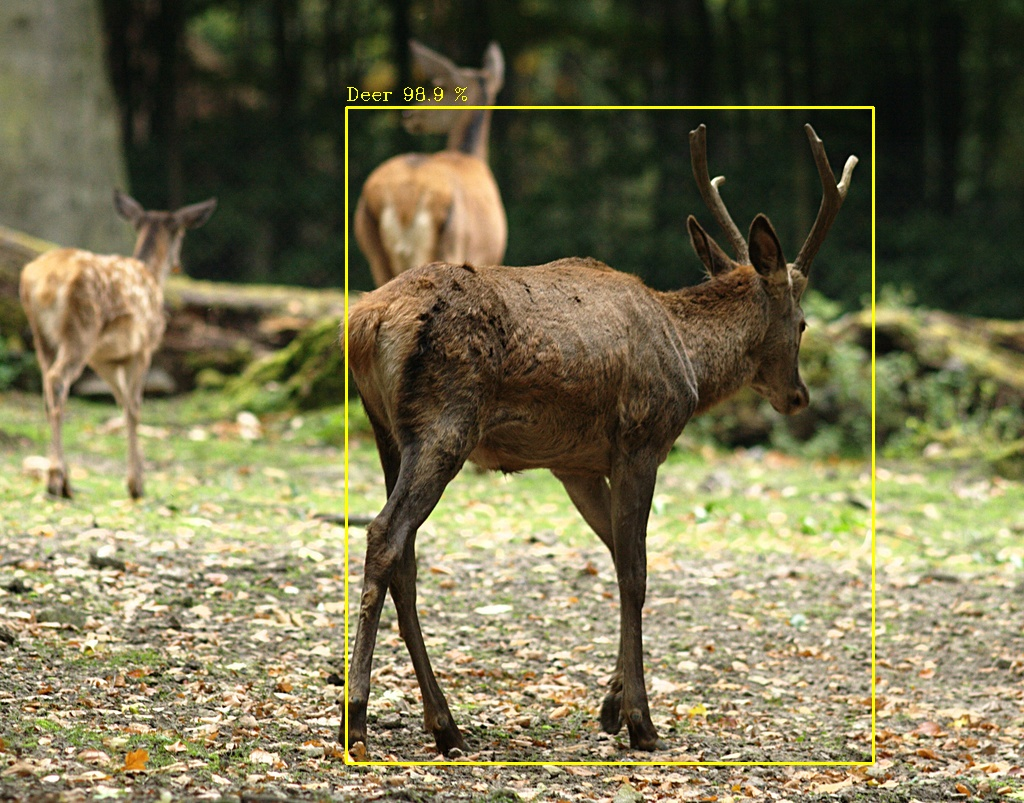
\includegraphics[width=0.9\textwidth]
  {model_compare_test__ssd_inception_v2.jpg}
  \captionof{figure}{SSD}
  \label{fig:infer_res_ssd}
\end{minipage}
\begin{minipage}{0.5\textwidth}
  \centering
  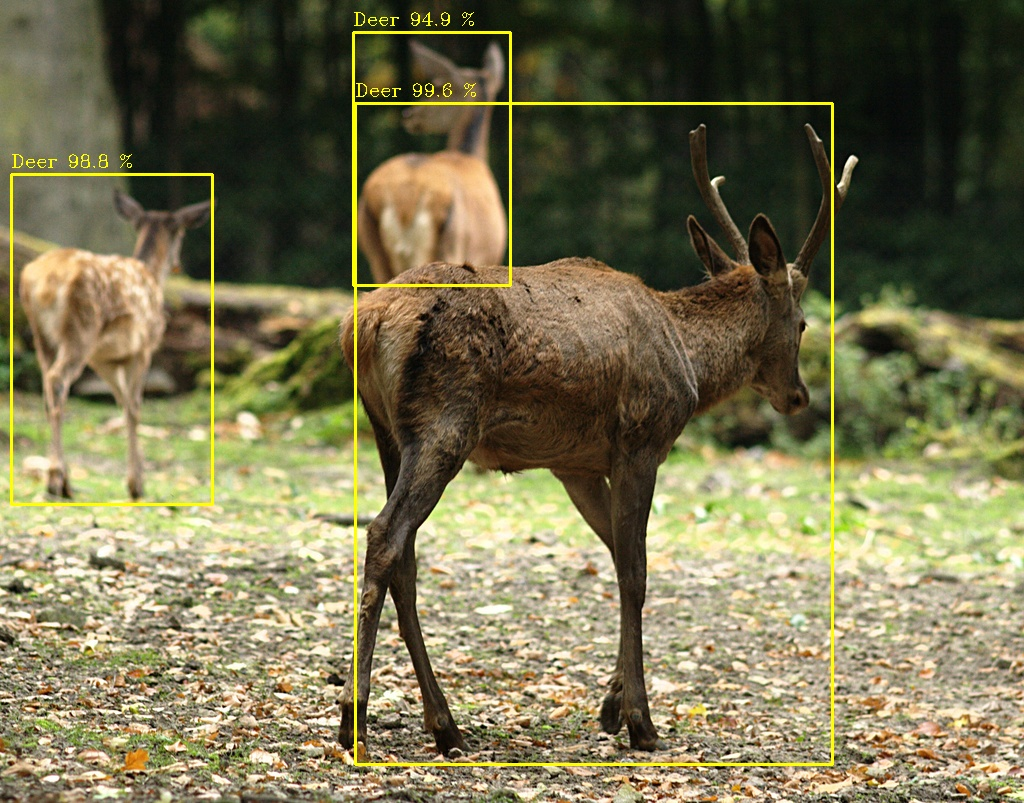
\includegraphics[width=0.9\textwidth]
  {model_compare_test__faster_rcnn_inception_v2_early_stopping.jpg}
  \captionof{figure}{Faster R-CNN}
  \label{fig:infer_res_faster_rcnn}
\end{minipage}


\subsubsection{Eigene Aufnahmen}

Bei der Inferenz, auf die eigenen Bilder, 
war ein deutlicher Unterschied der Modelle festzustellen.

In aufsteigender Reihenfolge lieferten das SSD mit MobilenetV2,
das SSD mit InceptionV2, das Faster R-CNN mit 
Early Stopping und Faster R-CNN mit Augmentierten Daten
wie in den Abbildungen \ref{fig:infer_res_ssd_mobile}
bis \ref{fig:infer_rest_rcnn_aug} zu sehen ist, 
bessere Ergebnisse.

Auch hier fiel auf, dass Tiere, die weiter weg und 
damit kleiner abgebildet sind,
besser von den Faster R-CNN Modellen
erkannt wurden.

\vspace{1cm}
\begin{minipage}{0.5\textwidth}
  \centering
  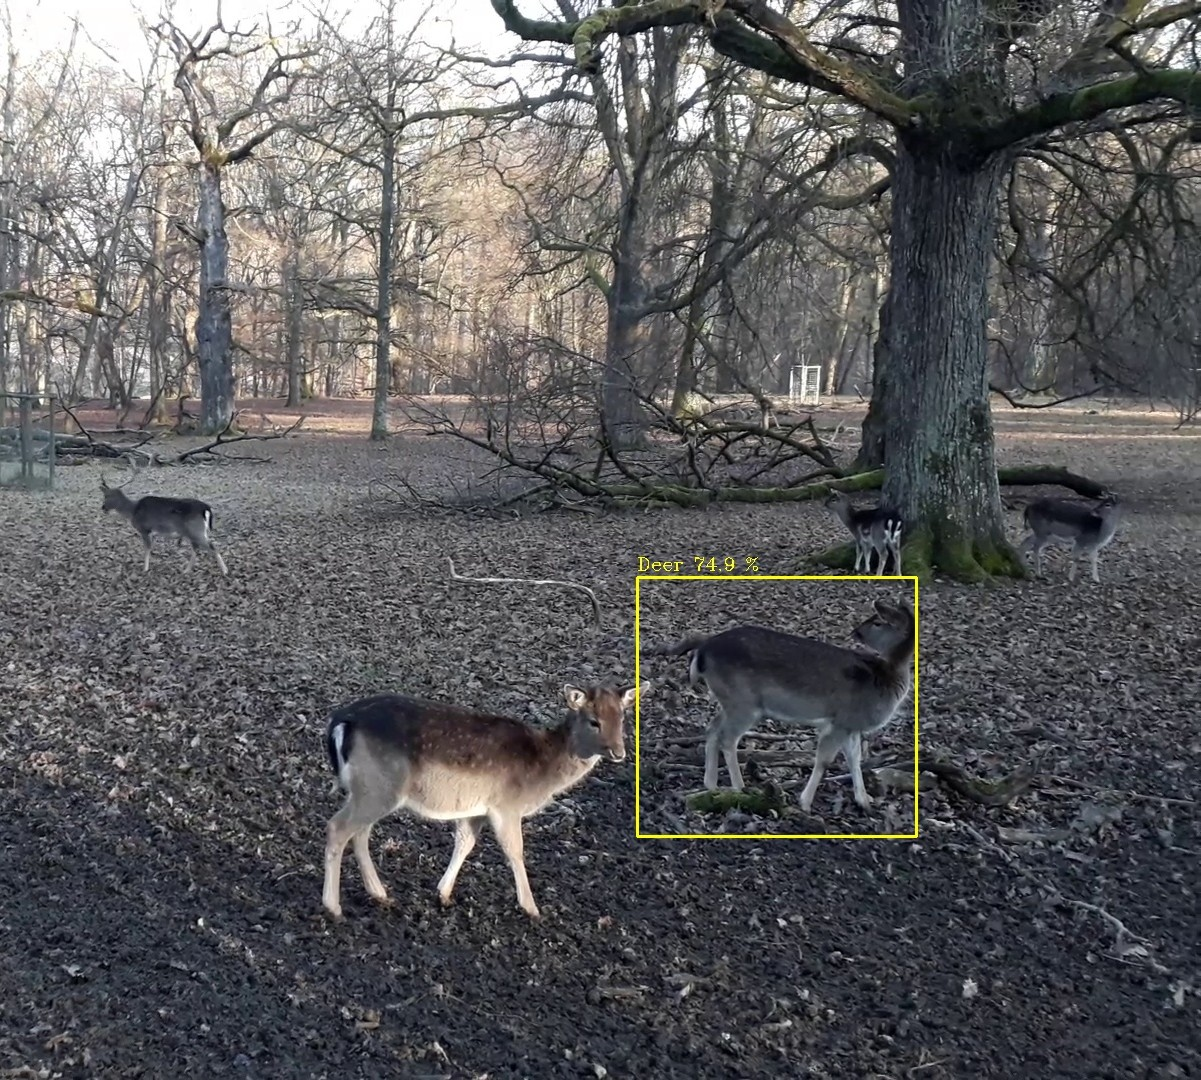
\includegraphics[width=0.9\textwidth]
  {model_compare_handy_ssd_mobilenet_v2.jpg}
  \captionof{figure}{SSD Mobilnet}
  \label{fig:infer_res_ssd_mobile}
\end{minipage}
\begin{minipage}{0.5\textwidth}
  \centering
  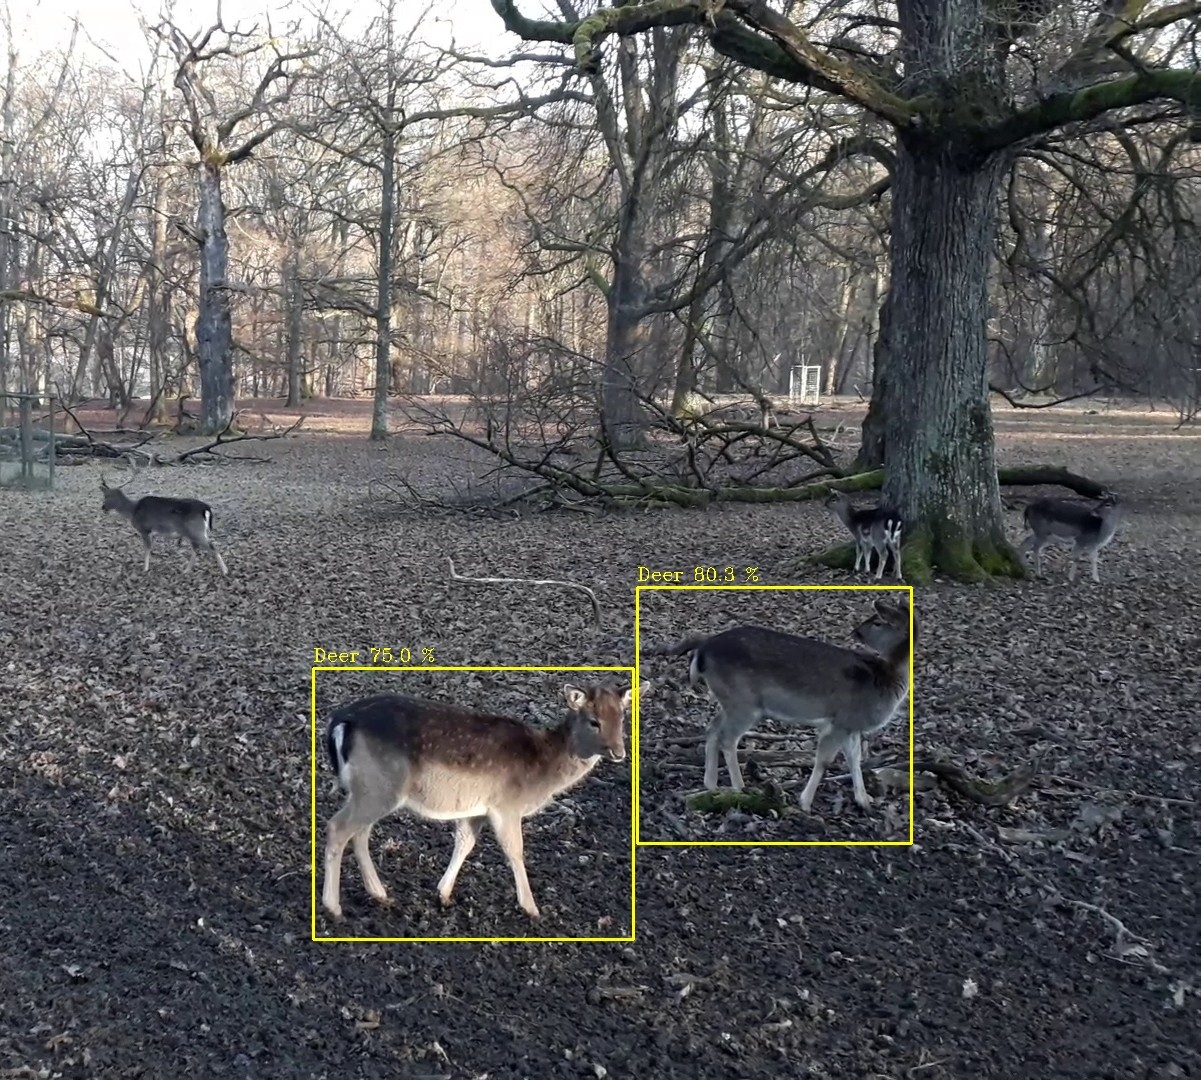
\includegraphics[width=0.9\textwidth]
  {model_compare_handy_ssd_inception_v2.jpg}
  \captionof{figure}{SSD Inception}
  \label{fig:infer_res_ssd_inception}
\end{minipage}
\\[1cm]
\begin{minipage}{0.5\textwidth}
  \centering
  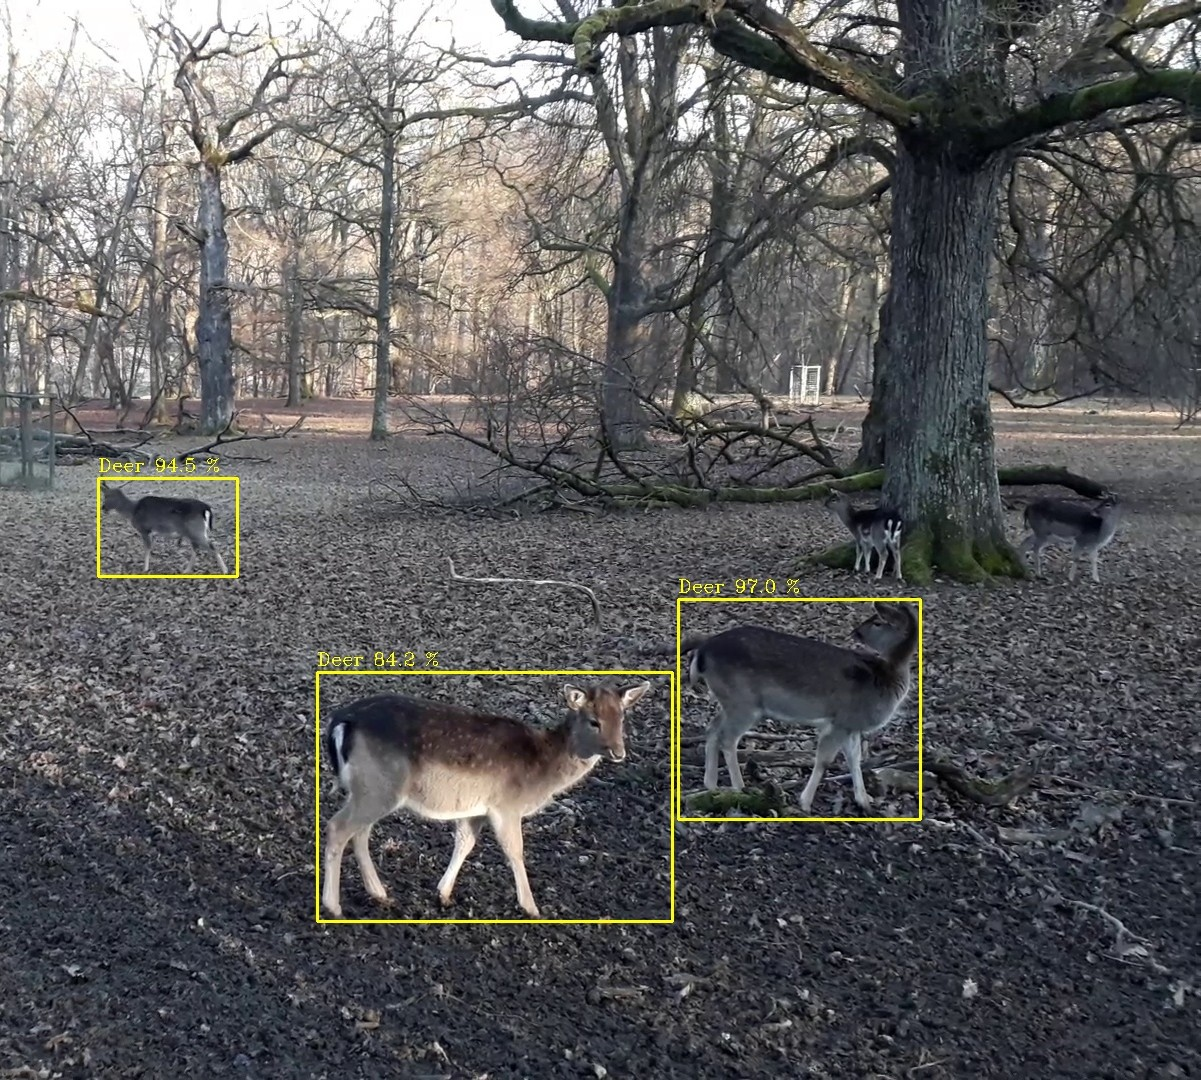
\includegraphics[width=0.9\textwidth]
  {model_compare_handy_faster_rcnn_inception_v2_early_stopping_ohne_aug.jpg}
  \captionof{figure}{Faster R-CNN mit Early Stopping}
  \label{fig:infer_res_rcnn_early_stopping}
\end{minipage}
\begin{minipage}{0.5\textwidth}
  \centering
  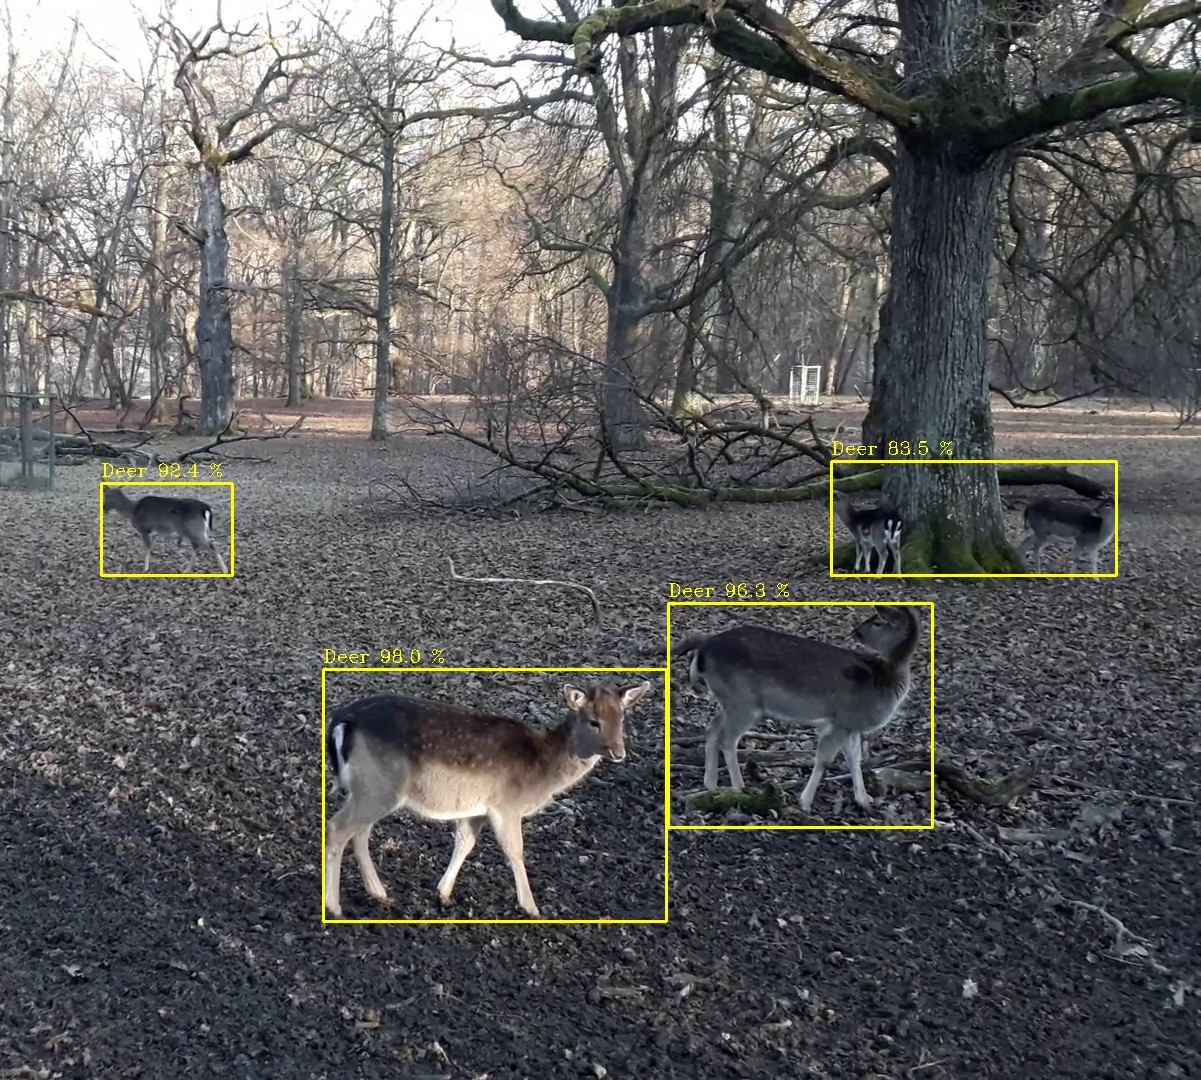
\includegraphics[width=0.9\textwidth]
  {model_compare_handy_faster_rcnn_inception_v2_early_stopping.jpg}
  \captionof{figure}{Faster R-CNN mit Augmentierung}
  \label{fig:infer_rest_rcnn_aug}
\end{minipage}



\subsubsection{iWildCam Datensatz}

Aus dem \textit{iWildCam 2019 Dataset}, welches aus einer 
\textit{Kaggle} Competition stammt, wurden die Klassen, welche
sich mit den für das Training verwendeten
überschnitten, für die Test Inferenz heruntergeladen.
Bei den Bildern handelt es sich um Aufnahmen von
Wildtier Kameras, aus dem Süd- und Nordwesten Amerikas,
welche aus der \textit{iNaturalist} und der \textit{Microsoft
DatAirSim} Datenbank stammen.

Darunter enthalten sind viele Nachtaufnahmen, welche teils 
schlecht beleuchtet und mit einer Infrarot Kamera aufgenommen und daher 
in Graustufen sind.

Da die Inferenzergebnisse hier bei allen vier Model Variationen 
deutlich schlechter, als bei den anderen Datensätzen war, 
wurde versucht dieses, durch weitere Optimierungen, zu verbessern.


%----------------- SECTION: optimierung ---------------------
\section{Optimierungen: Faster R-CNN}
\label{sec:optimierung_faster_rcnn}

Als Ausgangslage zur Verbesserung der Ergebnisse diente 
das Faster R-CNN mit augmentiertem Datensatz, welches
bei der Evaluierung im vorherigen Abschnitts die besten
Resultate erzielte.

Die Auswertung erfolgt hier wieder zunächst 
anhand der Evaluierungsmetriken und der Trainingsverläufe
aus Tensorboard und anschließend anhand der,
auf Testbilder ausgeführten, Inferenzergebnisse.



\subsection{Verschiedene Augmentierungen}

Der erste Ansatz zur Verbesserung der Ergebnisse war es,
das Faster R-CNN mit unterschiedlich starker Augmentierung
der Daten, für insgesamt mehr Iterationen
(500k statt 200k), zu trainieren.

Dabei wurde wieder das im Abschnitt \ref{subsec:augmentation} 
erläuterte Augmentierungsverfahren angewendetet, mit zusätzlich 
folgenden Variationen:

\begin{enumerate}
  \item Nur eine zufällige Augmentierung pro Bild, (anstelle von zwei)
  \item 4000 Bilder pro Klasse generieren (anstelle von 3000) 
\end{enumerate}

Die Trainingsergebnisse für 500k Iterationen sind anhand der 
Trainingsverläufe von Loss und mAP in den Abbildungen
\ref{plot:map_diff_aug} und \ref{plot:loss_diff_aug} dargestellt.

\vspace{1cm}
\begin{minipage}{0.5\textwidth}
  \centering
  \def\svgwidth{0.9\textwidth}
  \input{Bilder/plots/diff_aug_map.pdf_tex}
  \captionof{figure}{mAP}
  \label{plot:map_diff_aug}
\end{minipage}
\begin{minipage}{0.5\textwidth}
  \centering
  \def\svgwidth{0.9\textwidth}
  \input{Bilder/plots/diff_aug_loss.pdf_tex}
  \captionof{figure}{Loss}
  \label{plot:loss_diff_aug}
\end{minipage}

% Legende
% orange: FF7043
% blue  : 0077BB
% red   : CC3311
\begin{table}[htb]
  \centering
  \begin{tabular}{ m{0.4\textwidth}<{\centering}
                   m{0.2\textwidth}<{\centering}
                   m{0.2\textwidth}<{\centering}}
      $\color[HTML]{CC3311}\medbullet$ nur eine Augmentierung je Bild &
      $\color[HTML]{FF7043}\medbullet$  3000 Bilder &
      $\color[HTML]{0077BB}\medbullet$  4000 Bilder
  \end{tabular}    
\end{table}
\vspace{1cm}

Aufgrund des länger durchgeführten Trainings
ist bei allen Konfigurationen im, gegensatz zu den
Ergebnissen des vorherigen Abschnitts, Overfitting 
festzustellen.

Dieses fällt, wie zu erwarten war, bei den weniger  
augmentierten Datensätzen stärker aus, welche auf der 
anderen Seite einen besseren mAP Wert erreichen konnten.

Ob sich, konkret für diesen Fall, ein höherer mAP oder 
besserer Loss Wert positiver auf das Ergebnis auswirkt,
konnte wieder mithilfe der Inferenz auf Testbilder 
herausgefunnden werden.

\vspace{1cm}
\begin{minipage}{0.333\textwidth}
  \centering
  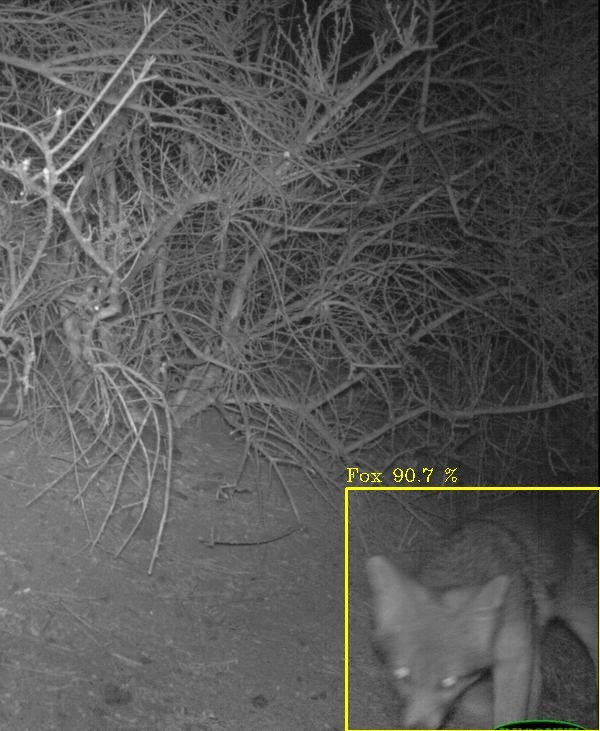
\includegraphics[width=\textwidth]{infer_images/iWildCam/fox/cut/59df5ee1-23d2-11e8-a6a3-ec086b02610b_faster_rcnn_inception_v2_3000.jpg}
  \captionof{figure}{3000 Samples}
  \label{fig:infer_res_3000}
\end{minipage}
\begin{minipage}{0.333\textwidth}
  \centering
  \label{fig:infer_res_4000}
  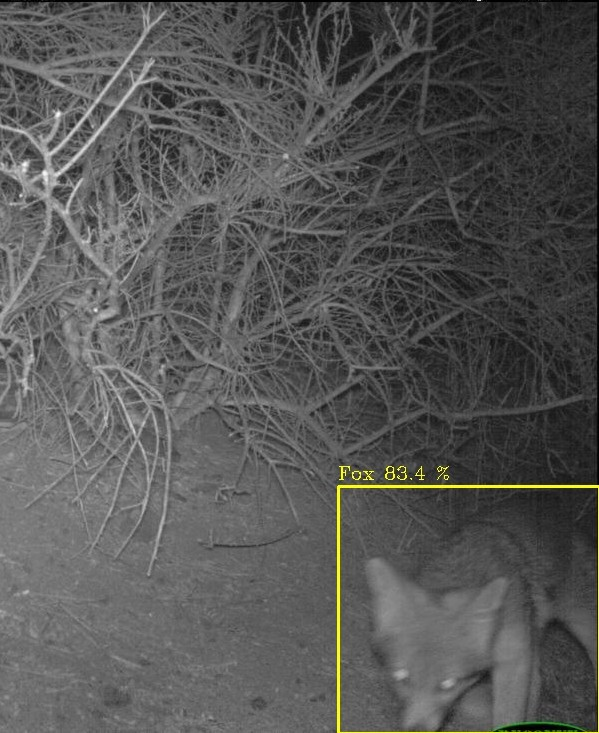
\includegraphics[width=\textwidth]{iWildCam/fox/cut/59df5ee1-23d2-11e8-a6a3-ec086b02610b_faster_rcnn_inception_v2_4000.jpg}
  \captionof{figure}{4000 Samples}
\end{minipage}
\begin{minipage}{0.333\textwidth}
  \centering
  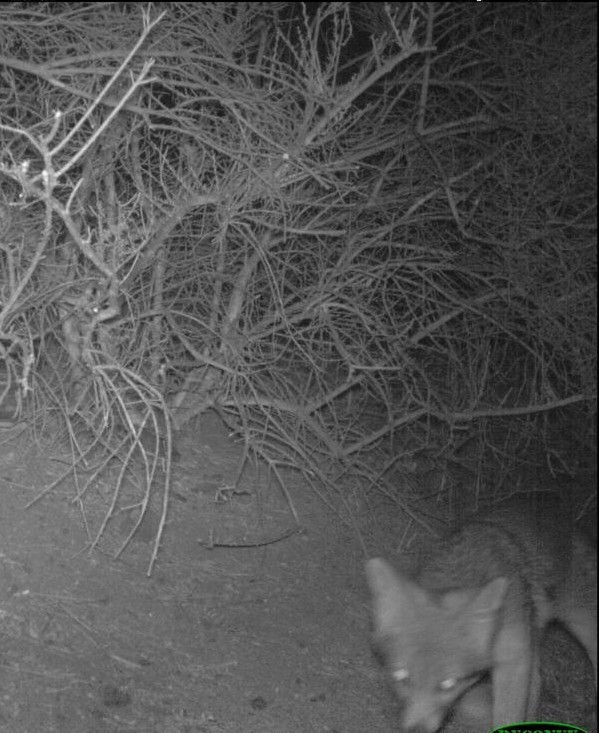
\includegraphics[width=\textwidth]{iWildCam/fox/cut/59df5ee1-23d2-11e8-a6a3-ec086b02610b_faster_rcnn_inception_v2_less_aug.jpg}
  \captionof{figure}{50\% Augment}
  \label{fig:infer_rest_05}
\end{minipage}
\vspace{1cm}

Abbildung \ref{fig:infer_res_3000} bis \ref{fig:infer_rest_05}
zeigen beispielhaft die Inferenzergebnisse für Bilder des 
\textit{iWildCam} Datensatzes, bei dem sich diesesmal der 
Unterschied deutlicher bemerkbar machte.
Das, auf weniger stark augmentierte Daten trainierte, 
Modell konnte die Tiere schlechter oder gar nicht erkennen.


\subsection{Verschiedene Regularisierungen}

Um das, trotz Augmentierung, zu stande kommende Overfitting zu 
vermeiden, wurde nun zusätzlich die L2 Regularisierung angewendet.
Diese soll, wie in den Grundlagen (Abschnitt \ref{subsec:validation})
beschrieben wurde, durch Anhängen einer Aufsummierung der Gewichte
an die Loss Funktion, ein Überanpassen des Modells an die
Trainingsdaten, reduzieren.

In der Konfigurationsdatei des Fater R-CNN kann dies,
durch setzten eines bestimmten Parameters für, sowohl die
erste Stufe des Modells, dem Region Proposal Network (RPN),
als auch für die zweite Stufe, dem Klassifikationsmodell,
seperat eingestellt werden.

Ebenso lassen sich die beiden Losskurven, aus denen sich 
beim Faster R-CNN der gesammte Loss zusammensetz,
seperat anzeigen, was in den Verläufen in 
Abbildung \ref{plot:aug_l2_classifier_loss}
und \ref{plot:aug_l2_rpn_loss} dargestellt ist.

Durch die getrennte Beobachtung der Loss-Kurven ließ sich 
feststellen, dass das Overfitting nur das RPN betrifft,
weshalb der Parameter zur L2 Regulierung nur 
für die erste Stufe eingestellt wurde.
Dafür wurde der Faktor $\lambda = 0.01$ gesetzt.

Vergleicht man nach dem Training mit 
reguliertem Modell wieder die Losskurven, ist deutlich zu 
erkennen, dass sich das Overfitting im RPN 
reduzieren ließ, wodurch sich auch der
in Abbildung \ref{plot:aug_l2_total_loss} 
dargestellte gesammt Loss verbesserte.

Die Verbesserung des Loss Wertes 
ging hier wieder mit einer leichten 
Verschlechterung des mAPs einher, wie in Abbildung
\ref{plot:aug_l2_mAP} zu erkennen ist.

\vspace{1cm}
\begin{minipage}{0.5\textwidth}
  \centering
  \def\svgwidth{0.9\textwidth}
  \input{Bilder/plots/aug_l2_mAP.pdf_tex}
  \captionof{figure}{mAP}
  \label{plot:aug_l2_mAP}
\end{minipage}
\begin{minipage}{0.5\textwidth}
  \centering
  \def\svgwidth{0.9\textwidth}
  \input{Bilder/plots/aug_l2_total_loss.pdf_tex}
  \captionof{figure}{Total Loss}
  \label{plot:aug_l2_total_loss}
\end{minipage}
\\[1cm]
\begin{minipage}{0.5\textwidth}
  \centering
  \def\svgwidth{0.9\textwidth}
  \input{Bilder/plots/aug_l2_classifier_loss.pdf_tex}
  \captionof{figure}{Klassifikations Loss}
  \label{plot:aug_l2_classifier_loss}
\end{minipage}
\begin{minipage}{0.5\textwidth}
  \centering
  \def\svgwidth{0.9\textwidth}
  \input{Bilder/plots/aug_l2_rpn_loss.pdf_tex}
  \captionof{figure}{RPN Loss}
  \label{plot:aug_l2_rpn_loss}
\end{minipage}
\begin{table}[htb]
  \centering
  \begin{tabular}{m{0.3\textwidth}<{\centering}
                  m{0.4\textwidth}<{\centering}}
     $\color[HTML]{CC3311}\medbullet$  nur Augmentierung &
     $\color[HTML]{0077BB}\medbullet$  Augmentierung + L2 Regularisierung
  \end{tabular}    
\end{table}
\vspace{1cm}

Auch hier wurde, zur Feststellung der Auswirkung 
der Unterschielichen Ergebnisse, wieder die 
Testinferenz angewendet, was beispielhaft 
für Bilder der eigenen Aufnahmen in den 
Abbildungen \ref{fig:test_infer_normal_aug}
und \ref{fig:test_infer_aug_plus_l2} dargestellt ist.


\vspace{1cm}
\begin{minipage}{0.5\textwidth}
  \centering
  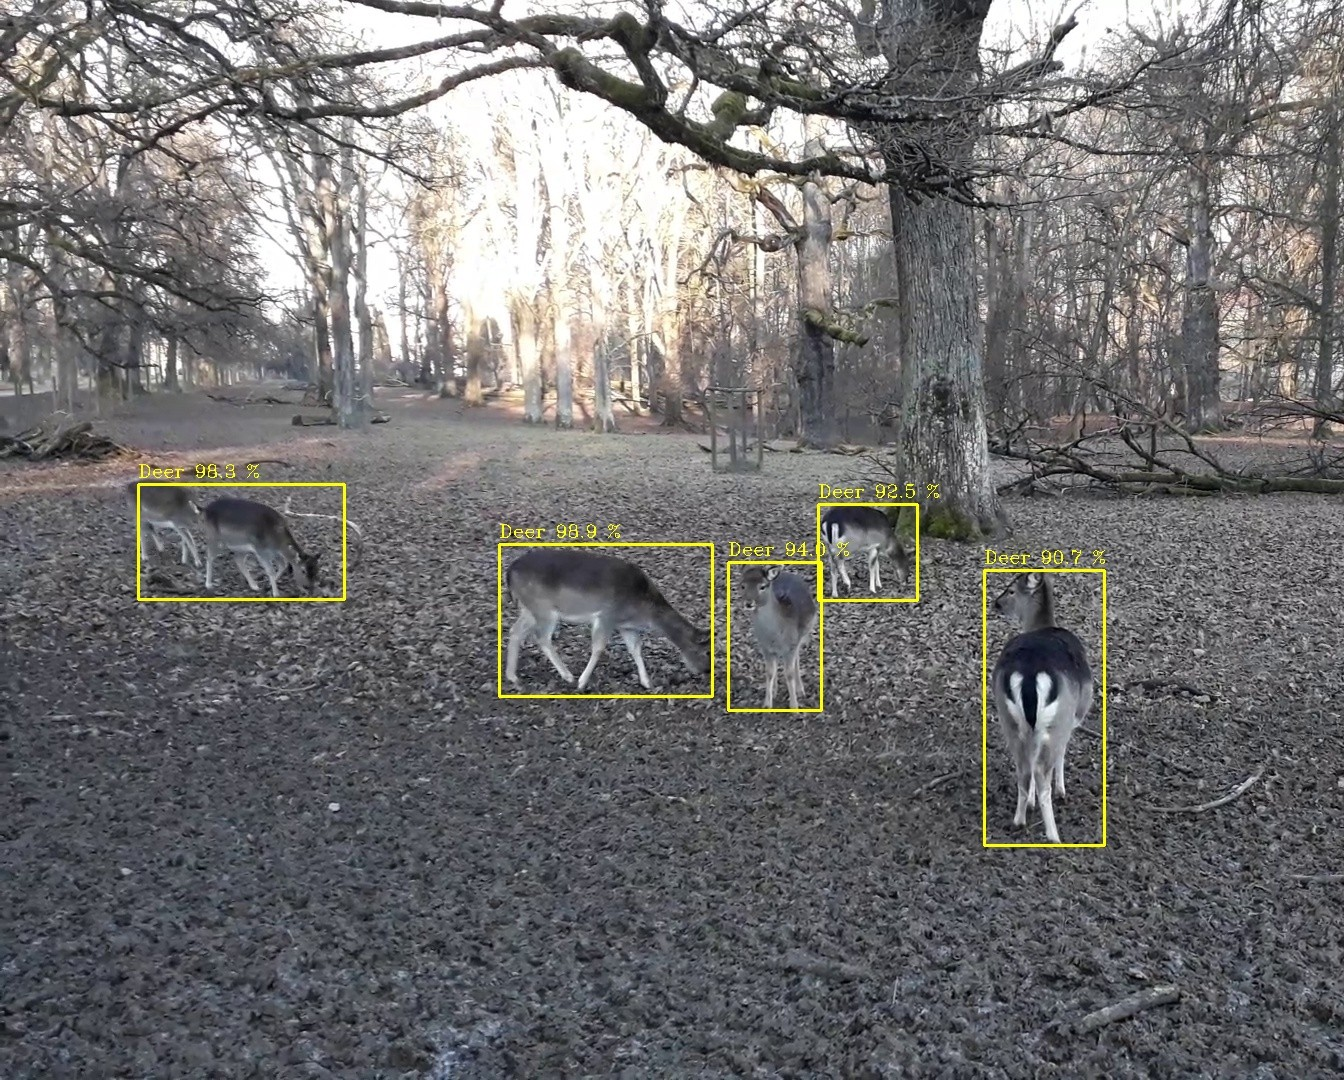
\includegraphics[width=0.95\textwidth]
  {eigene/20191229_145616_frame_20_faster_rcnn_inception_v2_3000.jpg}
  \captionof{figure}{Augmentierung (normal)}
  \label{fig:test_infer_normal_aug}
\end{minipage}
\begin{minipage}{0.5\textwidth}
  \centering
  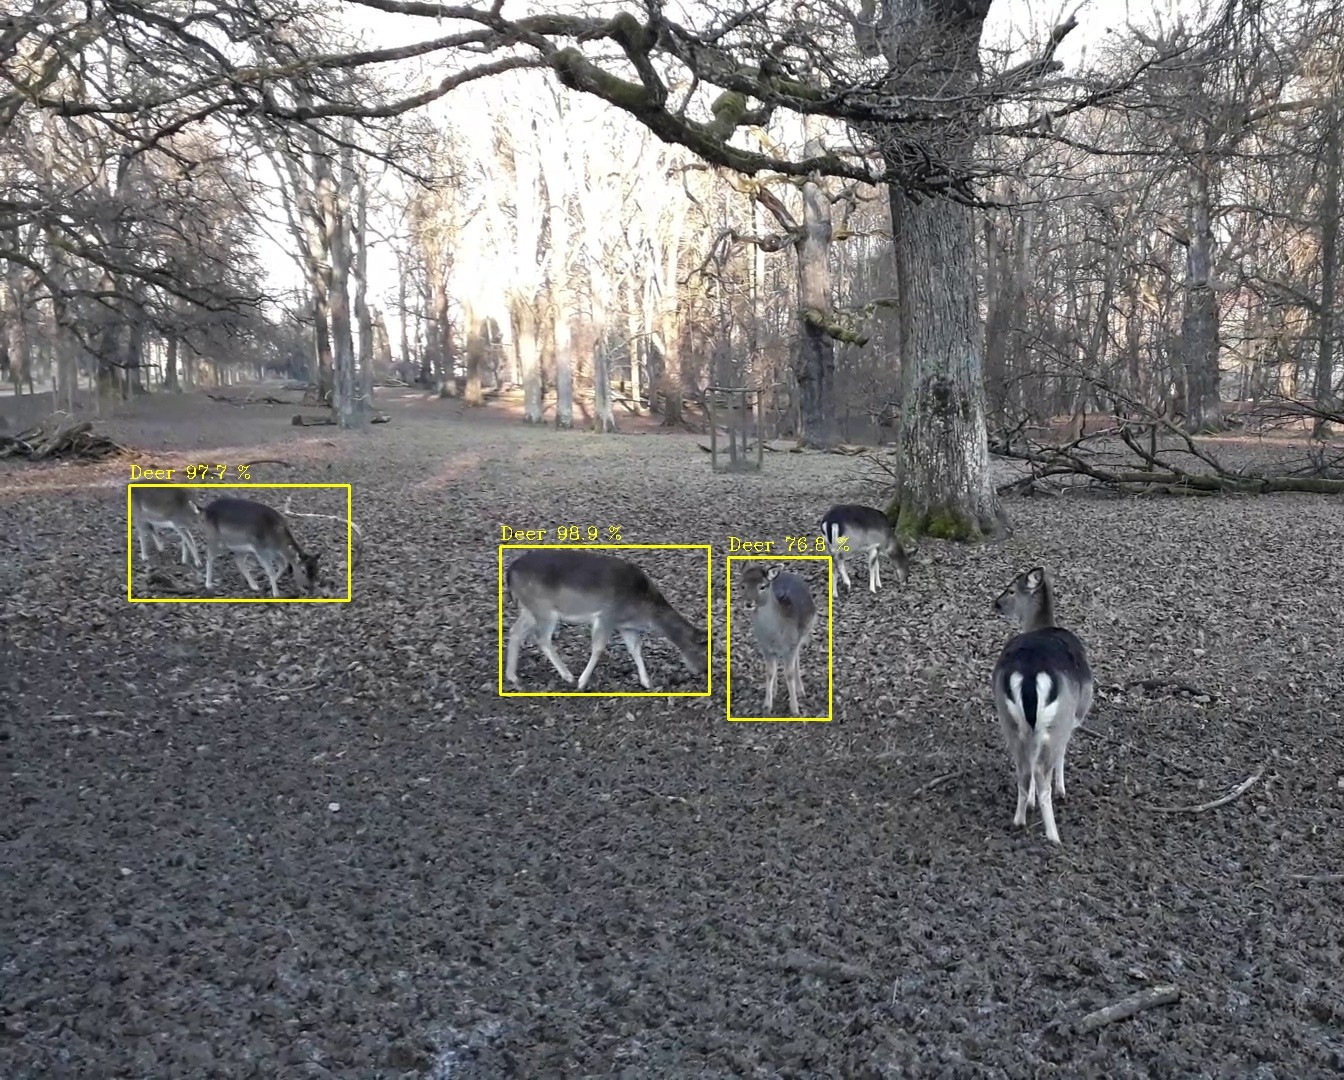
\includegraphics[width=0.95\textwidth]
  {eigene/20191229_145616_frame_20_faster_rcnn_inception_v2_l2.jpg}
  \captionof{figure}{Augmentierung + L2}
  \label{fig:test_infer_aug_plus_l2}
\end{minipage}
\vspace{1cm}

Hier ergaben die Inferenzergebnisse, dass 
eine L2 Regulierung der Modelle
in den meisten Fällen keinen Einfluss auf das Ergebnis
hat, falls doch, dieses sich tendentiell sogar
verschlechterte.

Weitere angewendete Regularisierungen, die jedoch 
auch zu keiner nennenswerten Veränderung der Trainingsergebnisse
führten, waren Dropout sowie L2 mit $\lambda = 0,02$ und sind in 
Tabelle \ref{table:reg}, zusammen mit den anderen Ergebnissen
dargestellt.


\vspace{1cm}
\begin{table}[htb]
  \centering
  \begin{tabular}{m{0.35\textwidth}|m{0.25\textwidth}<{\centering}m{0.25\textwidth}<{\centering}}
  \hline
                    & mAP  & Loss  \\ \hline\hline
  Augmentierung (50\%) &  0,72    &    0,76   \\
   + L2 Reg. ($\lambda = 0,01$)            &   0,71     & 0,75       \\\hline
  Augmentierung (normal)     & 0,7  & 0,74            \\
  + Dropout          & 0,7  & 0,73            \\
  + L2 Reg. ($\lambda = 0,01$)    & 0,7  & 0,69            \\
  + L2 Reg. ($\lambda = 0,02$)    & 0,69 & 0,7             \\ \hline
  Augmentierung (4000 Samples) &0,7&0,71\\\hline
  \end{tabular}
  \caption{Regularisierungen}
  \label{table:reg}
\end{table}
\vspace{1cm}

Aus den Ergebnissen ließ sich schließen, dass die Art
der Aufbereitung der Daten den größeren Einfluss auf die Ergebnisse
haben und durch Anpassungen der Hyperparameter, wenn überhaupt,
nur noch geringfügige Optimierungen betrieben werden können.
So hat insgesammt das Faster R-CNN, mit 500k Trainingsiterationen 
auf Augmentierte Daten mit 3000 Bildern je Klasse, zu
den besten Ergebnissen, bezüglich Genauigkeit, geführt.


\section{Inferenzzeit}\label{sec:infertime}

Neben der Genauigkeit, war die Ausführungszeit, welche ein Model für die 
Inferenz benötigt, ein weiteres Kriterium für die Auswahl des, in 
der Anwendung zu verwendenen, Modells.
Einer der Faktoren, welcher die Inferenzzeit beeinflusst,
ist die Hardware, auf der die Inferenz stattfindet,
sowie die zur Implementierung verwendeten Library.

Die Hardware war mit dem Neural Compute Stick 2 festgelegt, als 
Library kommen dafür \textit{OpenCV} oder \textit{OpenVino}
in Frage, wobei mit \textit{OpenVino} die Möglichkeit 
zur asynchronen Inferenzausführung, sowie der Verwendung mehrerer,
parallel ausgeführter, Inferenz Requests besteht,
wodurch sich die Inferenzzeit optimieren lässt.

Ein weiter Faktor ist die Komplexität des CNNs sowie die 
für die Objekterkennung verwendete Modell Architektur.
Üblicherweise sind Komplexere Modelle, wie das Faster R-CNN,
zwar genauer, jedoch auch langsamer.

Um den Effekt, den die drei unterschiedlichen, 
für das Training verwendeten, Varianten SSD mit MobilenetV2, 
SSD mit InceptionV2 und Faster R-CNN mit InceptionV2 auf die
Inferenzzeit haben zu Untersuchen,
wurden diese durch Messen der Inferenz-FPS verglichen.

Dabei wurde die Asynchrone Inferenz mit unterschiedlicher Anzahl 
an Inferenz Requests verwendet, weshalb in diesem Abschnitt 
zunächst die Funktionsweise der synchronen- und asynchronen
Inferenzausfürung mit OpenVino erklärt wird.


\subsection{Synchrone- und Asynchrone Inferenz}

Wird die Inferenz im synchronen Modus ausgeführt, kann immer
nur entweder inferiert, oder das Vor- und 
Nachverarbeiten, der Bilder stattfinden.

Vorverarbeitung der Bilder beeinhaltet dabei
z.B. die Umwandlung des von der Kamera gelieferten 
Bildformats, in das für das jeweilige Model richtige 
Input Format.
Die Nachverarbeitung bezieht sich auf das Verwenden 
der Inferenz Ergebnisse in der Anwendung.

Die Implementierung der Inferenz in OpenVino erfolgt
dementsprechend Sequentiell, wie im Algorithmus
\ref{code:sync} als Pseudocode dargestellt ist.

Anhand des zeitlichen Ablaufs, dargestellt in Abbildung
\ref{fig:sync}, sind die Abschnitte, in denen
keine Inferez stattfinden kann, deutlich zu erkennen.

\vspace{1cm}
\begin{minipage}{0.1\textwidth}
  \hfill
\end{minipage}
\begin{minipage}{0.5\textwidth}
  \begin{algorithm}[H]
    \caption{Synchrone Inferenz}
    \label{code:sync}
    \begin{algorithmic}
    \WHILE{\TRUE}
        \STATE capture FRAME
        \STATE preprocess CURRENT InferRequest
        \STATE \textbf{start} CURRENT InferRequest
        \STATE \textbf{wait} for CURRENT InferRequest
        \STATE process CURRENT result
    \ENDWHILE
    \end{algorithmic}
  \end{algorithm}  
\end{minipage}
\begin{minipage}{0.4\textwidth}
  \centering
  \vspace{1cm}
  \def\svgwidth{0.5\textwidth}
  \input{Bilder/sy_asy_legend.pdf_tex}
\end{minipage}

\vspace{1cm}
\begin{figure}[H]
  \centering
  \def\svgwidth{0.9\textwidth}
  %\tikzset{
    desicion/.style={
        diamond,
        draw,
        text width=4em,
        text badly centered,
        inner sep=0pt
    },
    block/.style={
        rectangle,
        draw,
        text width=5em,
        text height=1em,
        text centered
    },
    arrow/.style={
        draw,
        >=latex,
        ->
    }
}


\begin{tikzpicture}

    \node(infer1) [block] {infer1};
    \draw[arrow] (0,-1em) -- (10,-1em);
    % \node (A) [desicion] {entschei\\dung};
    % \node (B) [block, below of=A, node distance=5cm, text width=5em] {bock};
    % \node (C) [block, right of=A, node distance=5cm] {noch ein\\bock};


    % \draw[arrow] (A) --  node [left, fill=white] {yes} (B);
    % \draw[arrow] (A) -- node [below, near end] {crap} (C); 
    % \draw[arrow] (B) -| node [near start, fill=white] {yes} (C);

\end{tikzpicture}

  \input{Bilder/sync_infer.pdf_tex}
  \caption{}
  \label{fig:sync}
\end{figure}


Da die Inferenz auf dem Myriad Chip des Neural Compute Sticks
und nicht auf dem ausführenden Pc bzw. Raspberry Pi läuft,
kann diese ungehindert, parallel zum restlichen Programmablauf, 
erfolgen.

In OpenVino wird dieser Ablauf mithilfe der \textit{Asynchronen Api}
erreicht, welche, über einen bestimmten Funktionsaufruf,
die Inferenz in einem seperaten Thread startet.

Indem vor Erhalt und Verarbeitung eines aktuellen 
Inferenz Ergebnisses der Inferenz Request für
den nächsten Durchlauf aufgegeben wird, wie in Algorithmus
\ref{code:async} als Pseudocode dargestellt ist, kann der in
Abbildung \ref{fig:async} dargestellte Zeitliche Ablauf erreicht werden.


\vspace{1cm}
\begin{minipage}{0.1\textwidth}
  \hfill
\end{minipage}
\begin{minipage}{0.5\textwidth}
  \begin{algorithm}[H]
    \caption{Asynchrone Inferenz}
    \label{code:async}
    \begin{algorithmic}
    \WHILE{\TRUE}
        \STATE capture FRAME
        \STATE preprocess NEXT InferRequest
        \STATE \textbf{start} NEXT InferRequest
          \STATE \textbf{wait} for CURRENT InferRequest
          \STATE process CURRENT result
          \STATE swap CURRENT and NEXT InferRequest
    \ENDWHILE
    \end{algorithmic}
  \end{algorithm}
\end{minipage}
\begin{minipage}{0.4\textwidth}
  \centering
  \vspace{1cm}
  \def\svgwidth{0.5\textwidth}
  \input{Bilder/sy_asy_legend.pdf_tex}
\end{minipage}

\vspace{1cm}

\begin{figure}[H]
  \centering
  \def\svgwidth{0.9\textwidth}
  \input{Bilder/async_infer.pdf_tex}
  \caption{}
  \label{fig:async}
\end{figure}

Die hier mit \textit{Current} und \textit{Next} bezeichneten 
Inferenz Requests stehen für die Indizes der jeweiligen Requests
und können belieb erweitert werden. 
Dadurch wird erreicht, dass die Inferenz auf mehreren Threads 
parallel ausgeführt wird.
% https://docs.openvinotoolkit.org/2018_R5/_samples_object_detection_demo_ssd_async_README.html


\subsection{Vergleich der Modelle}

Mithilfe eines Python Scripts, in welchem die Asynchrone Inferenz 
für eine variabel einstellbare Anzahl an Inferenz Requests
implementiert wurde, konnte für die drei Modelle die 
durchschnittliche Anzahl an, pro Sekunde inferierten, Frames 
ermittelt werden.

Diese wurden auf dem Raspberry Pi mit dem Neural Compute Stick 
ausgeführt und lieferten die in Tabelle \ref{table:infertime}
dargestellten Ergebnisse.

\vspace{1cm}
\begin{table}[htb]
  \centering
  \begin{tabular}{m{0.25\textwidth}|m{0.1\textwidth}<{\centering}|m{0.1\textwidth}<{\centering}|m{0.1\textwidth}<{\centering}|m{0.1\textwidth}<{\centering}}
  \hline
  \multirow{2}{*}{Model} & \multicolumn{4}{c}{Asynchronge Inferenz Requests} \\ \cline{2-5} 
                         & 1           & 2          & 3          & 4          \\ \hline\hline
  SSD MobilenetV2        & 19,5           & 35,2          & 40,6          & 40,3          \\
  SSD InceptionV2        & 15,6           & 27,7          & 31,1          & 31,7          \\
  Faster R-CNN Incept.   & 0,63           & 0,67          & 0,75          & 0,74          \\ \hline
  \end{tabular}
  \caption{Vergleich von Inferenzzeiten der Modelle in FPS}
  \label{table:infertime}
\end{table}
\vspace{1cm}

Die asynchrone Inferenzausführung führte bei allen Modellen, 
für bis zu 3 inferenz Requests, zu besseren Ergebnissen.
Ein deutlicher Unterschied der Inferenzzeit war 
zwischen SSD und Faster R-CNN Architekuren festzustellen.

Da für die Anwendung zur Wildtiererkennung 
keine Realtime Performance erforderlich ist,
wurde durch geschickte Implementierung der Inferenz in der 
Applikation, trotz langsamerer Inferenzzeit, das 
Faster R-CNN verwendet.

%##########################  CHAPER 6: APPLICATION  #######################

\chapter{Entwicklung der Anwendung}\label{kap:application}


Dieses Kapitel beschreibt die Entwicklung der Anwendung,
welche als autonomes System dass auf einem Raspberry Pi 4 läuft.

Dazu gehören die Einrichtung einer infrarotfähigen 
Kamera, die Implementierung der Inferenz mit OpeVino
und die Verbindung zu einem Pc zur übertragung
der Daten mit geeignetem Protokolls.



%-------------------------  SECTION 1: AUFBAU  ------------------------
\section{Aufbau/Hardware}\label{sec:aufbau}


Der Aufbau besteht aus einem Raspberry Pi, auf welche 
der Anwendungscode läufr, dem NCS2 für die Inferenz, 
welcher per USB mit dem Raspberry verbunden wird.

Desweiteren wurde ein Raspberry Pi Kamera Modul mit 
5MP OV5647 Sensor der Marke Longrunner verwendet.

Dieses ermöglicht durch zu und abschalten eines Infrarot 
Filters vor die Linse zwischen Tag und Nachtsicht zu wechseln.

Das Schalten wird dabei über einen Helligkeitssensor automatisch 
geregelt. Im Infrarotmodus bfindet sich der Infrarot Filter nicht 
vor der linse, wodurch auch die etwas längeren (850nm)
Elektromagnetischen Wellen als die des Sichtbaren Lichts aufgenommen 
werden können.

Durch zwei Infrarot LEDs des gleichen Spektrums, können so 
auch in der Dunkelheit Bilder aufgenommen werden, ohne 
Sichtbare beläuchtung, was Tiere verscheuchen würde.


Das kamera Modul wird über die CSI (Camera Serial Interface) 
Schnittstelle mit dem Raspberry Pi verbunden.


%https://www.amazon.de/gp/product/B07R4JH2ZV/ref=ppx_yo_dt_b_asin_title_o01_s00?ie=UTF8&psc=1


\begin{minipage}{0.55\textwidth}
    \centering
    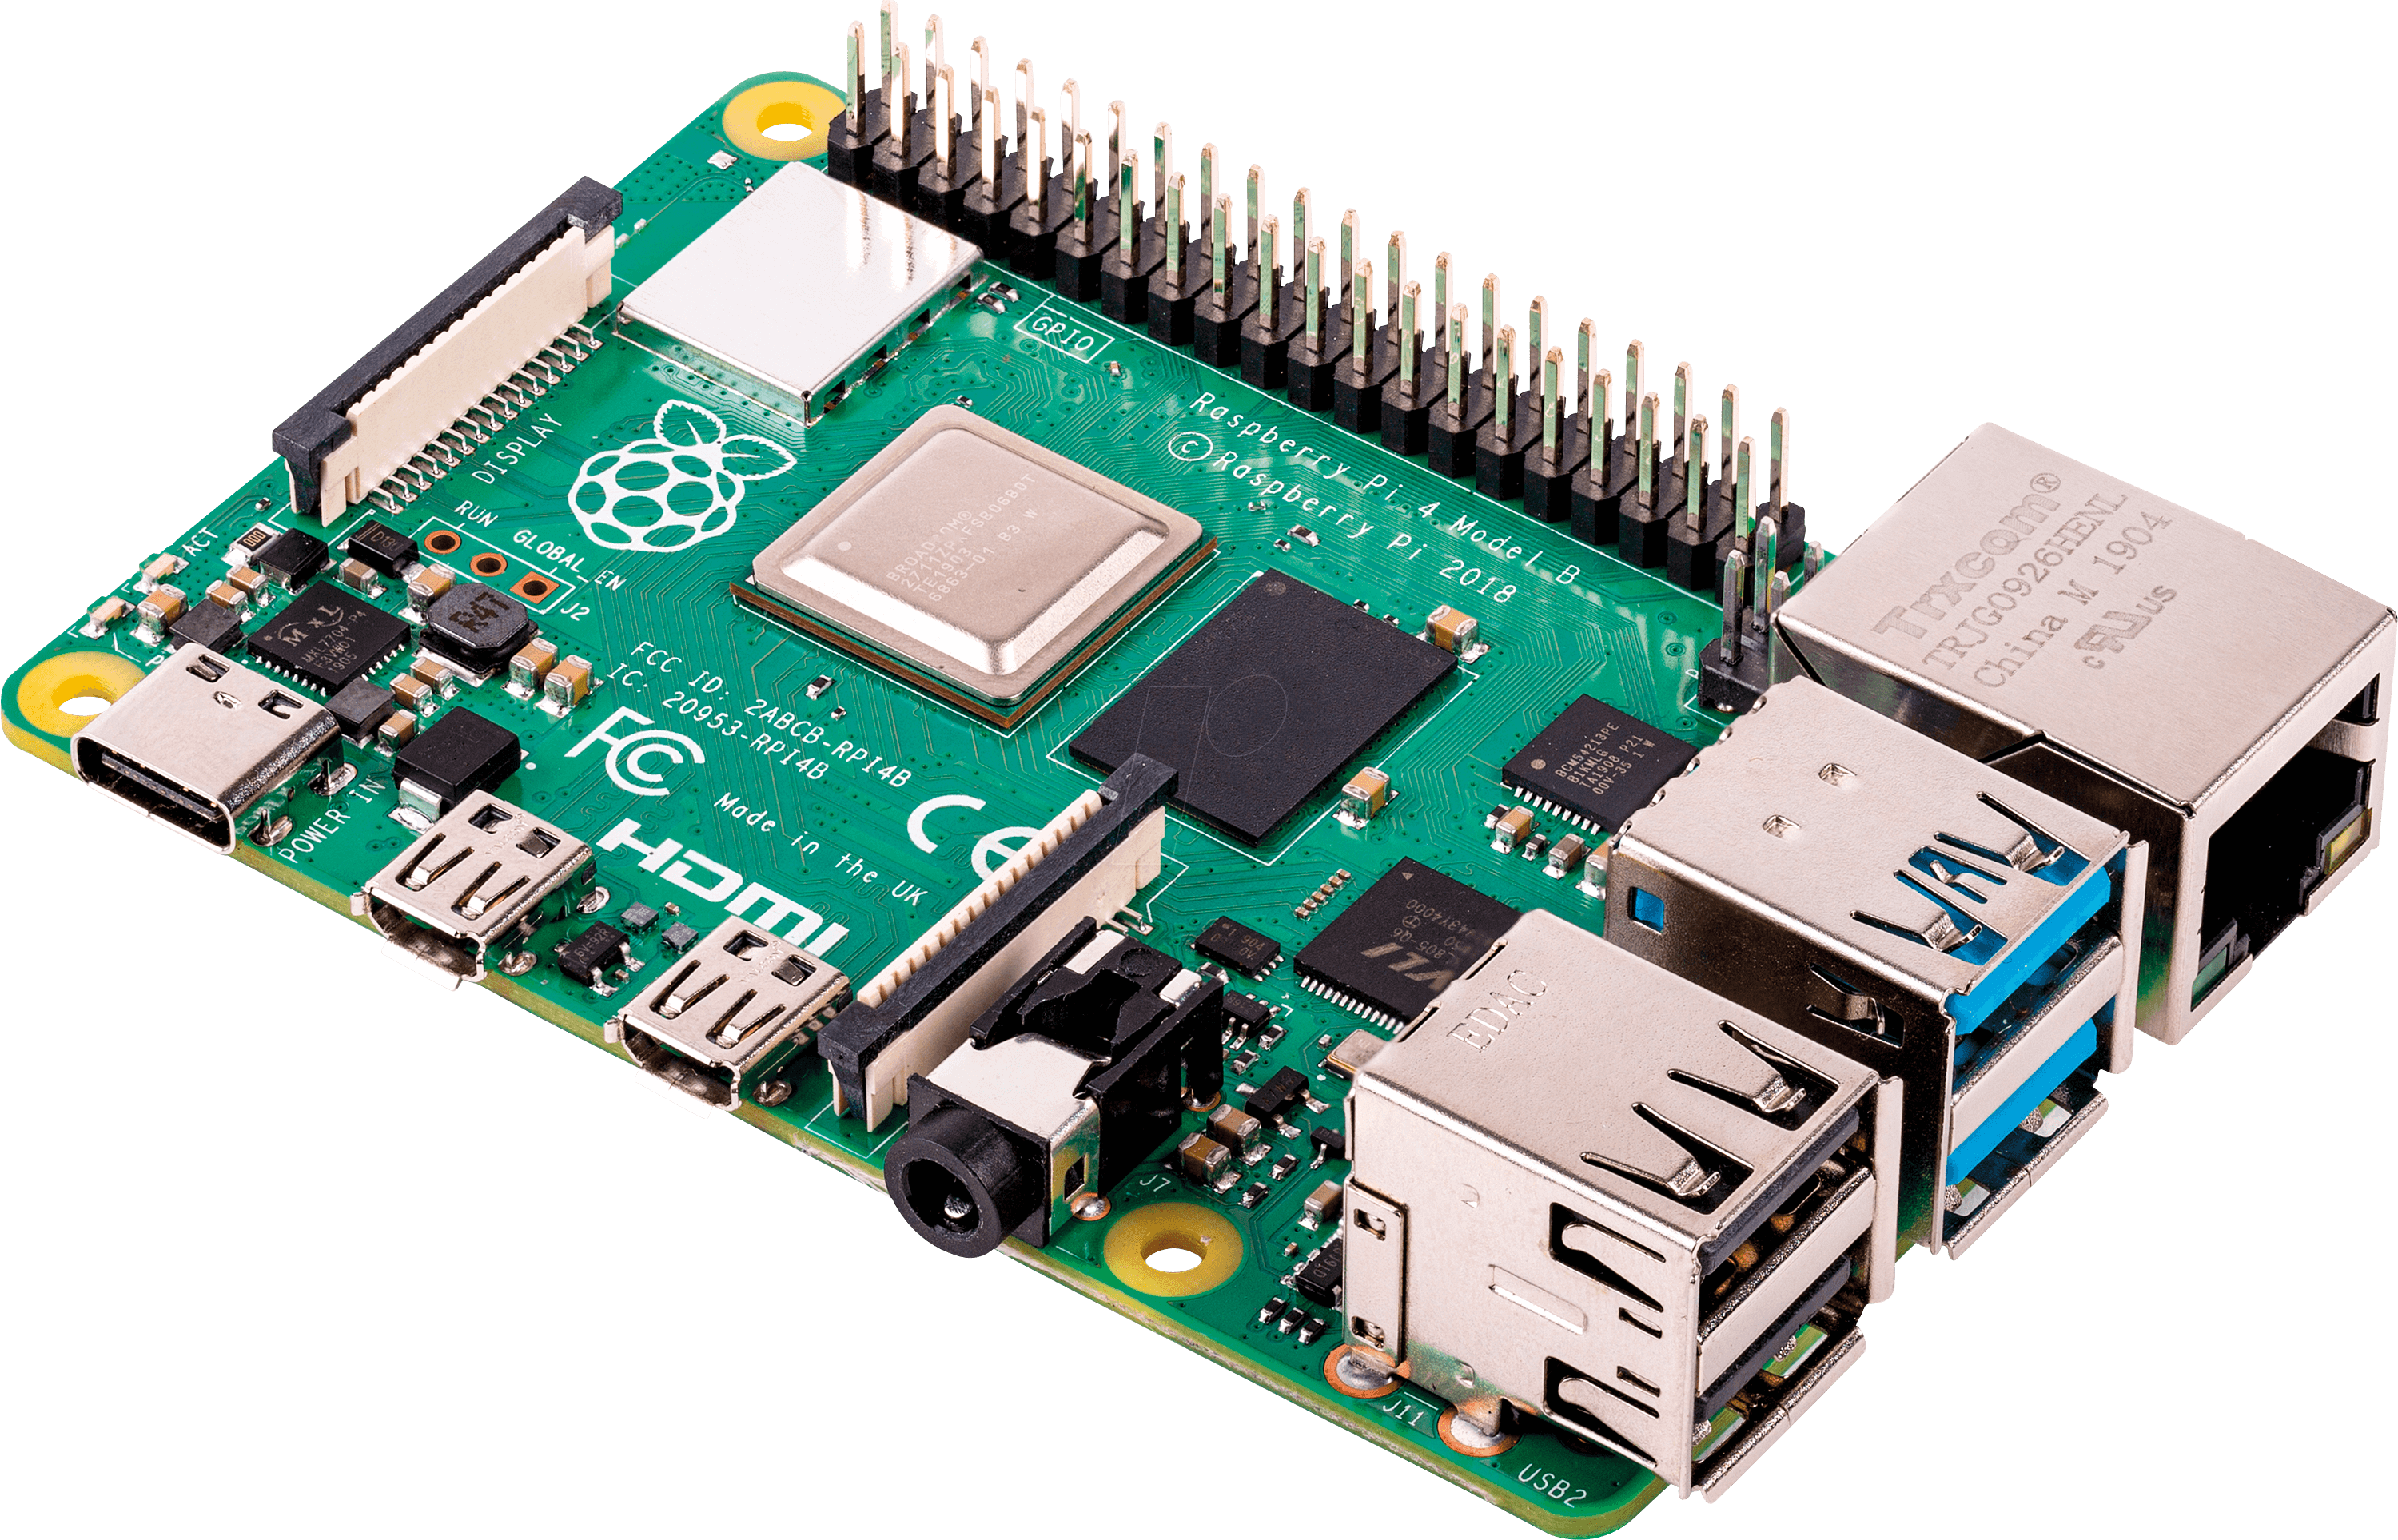
\includegraphics[width=0.8\textwidth]{./Bilder/raspberrypi_4.png}
    \captionof{figure}{Raspberry Pi 4}
    \label{img:raspberrypi}
\end{minipage}
\begin{minipage}{0.45\textwidth}
    \centering
    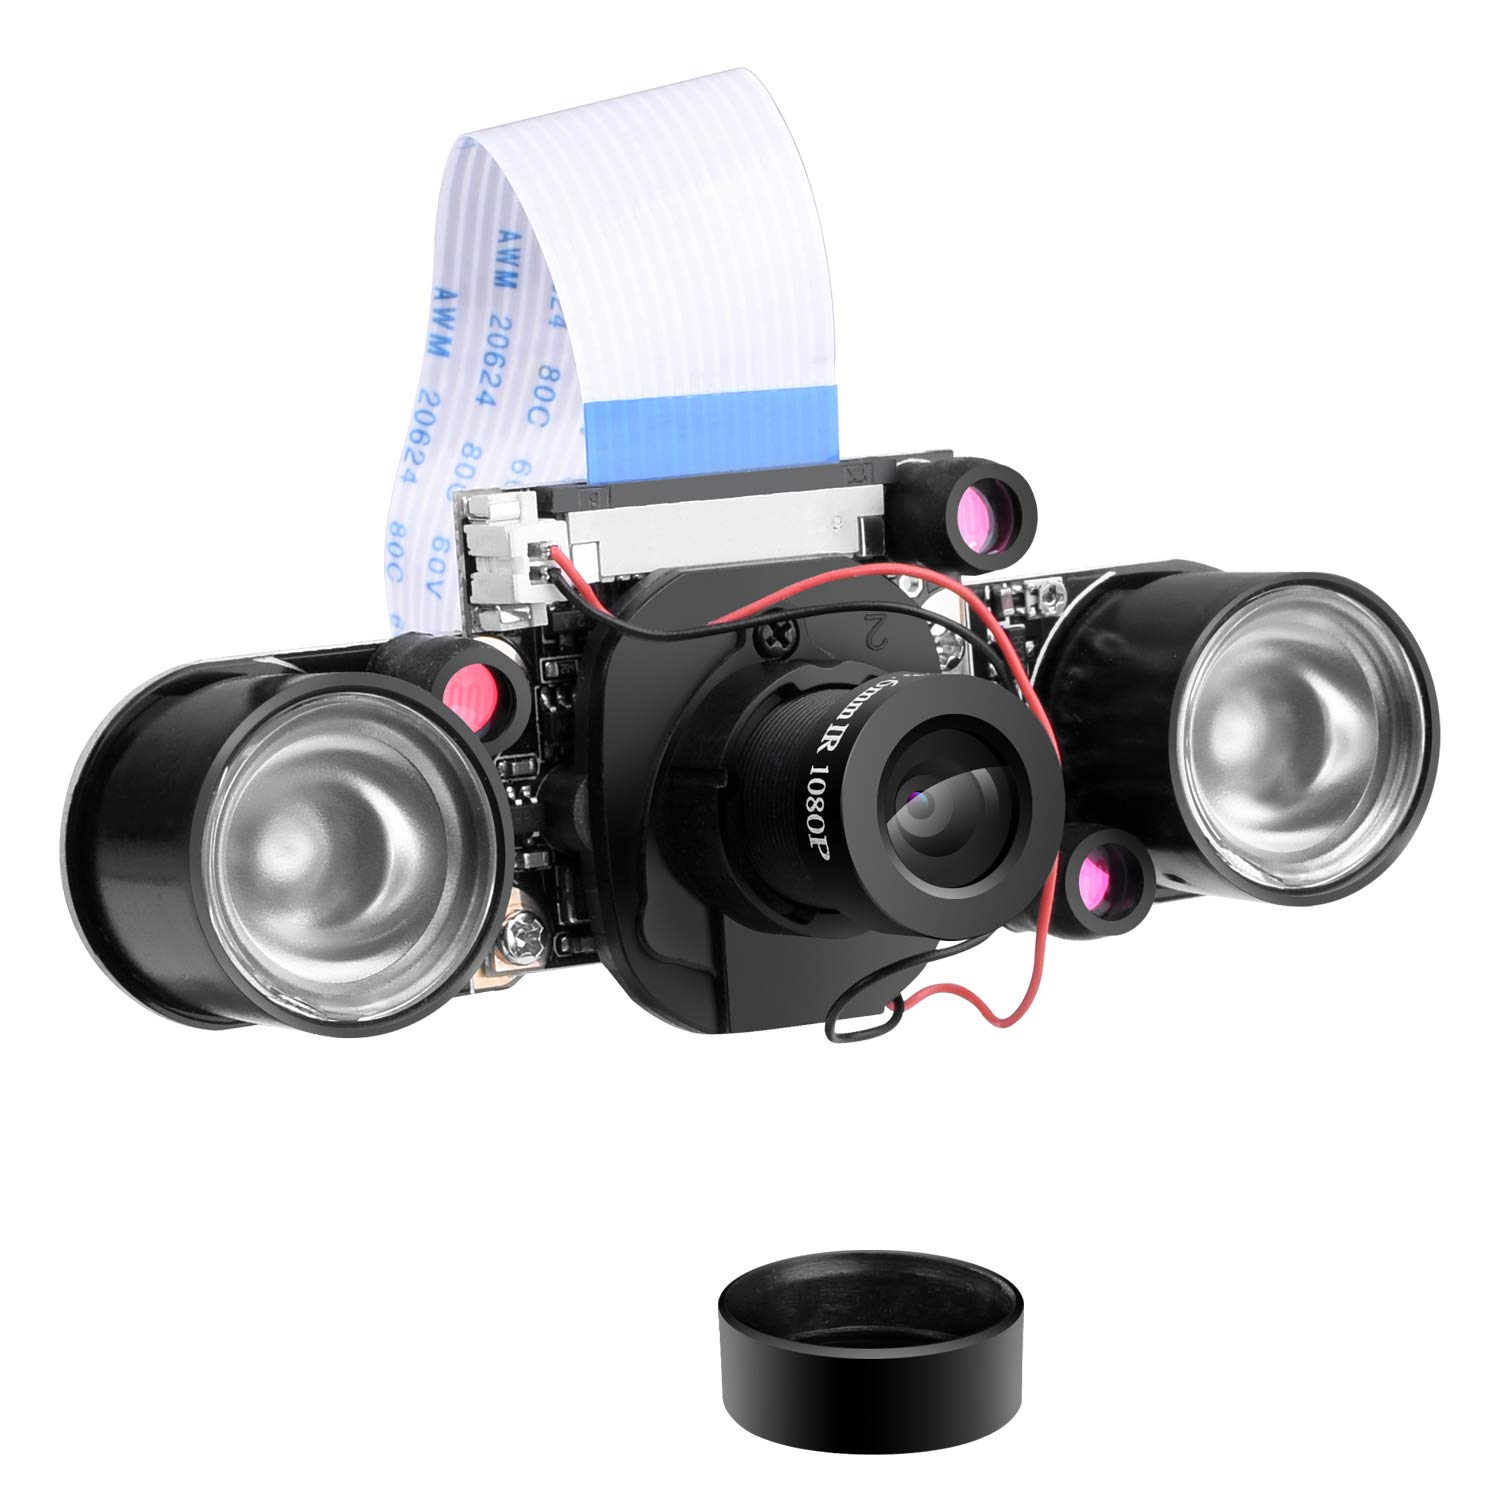
\includegraphics[width=0.8\textwidth]{longrunner.jpg}
    \captionof{figure}{Longruner Kamera Modul}
    \label{fig:rpicam}
\end{minipage}
\vspace{0.6cm}


Desweiteren wurde für eine mobile Internetverbindung 
der \textit{Huawei E3531 SurfStick} und zu Stromversorgnung
eine Powerbank verwendet.


% https://www.amazon.de/gp/product/B00HSZEY34/ref=ppx_yo_dt_b_asin_title_o00_s00?ie=UTF8&psc=1


\section{Implementierung/Software}

Die Implementierung der Anwendung wurde in Python vorgenommen und 
besteht aus den drei Scripten \texttt{main.py}, \texttt{detection.py}
und \texttt{connection.py}. Welche Folgend dargestellte Klassen 
implementieren.

\vspace{1cm}
\begin{tikzpicture} 

    
    
            \umlclass{Motion}{ 
              statickBackground : np.array
              }{ 
              + detectMotion() : bool \\
              + resetBackground() : void
            }
        
            \umlclass[y=-4]{InferenceModel}{ 
                string : plugin
                strin : device
                }{ 
                + createExecInferModel() : ExecInferModel
              }
        
            \umlclass[y=-2, x=6]{ExecInferModel}{ 
                shape : ioBlob\\
                detected : array
                }{ 
                + inferFrames() : status \\
                \# status[0] num infered\\
                \# status[1] num detected\\
                \# status[2] num saved\\
                - save() : void
                }
        
    
        \umlclass[x=11, y=-2]{Connection}{ 
            string logindata
            }{ 
            + login() : bool \\
            + connect() : server, port\\
            + send() : bool\\
            + disconnect() : bool\\
            + sendEmail(email, text) : boiol
          }

    
    \end{tikzpicture}
        
\vspace{1cm}

Dabei führt die Main Anwendung eine Dauerschleife aus, in der 
die Frames der Kamera erhalten werden. 

Die inferenz wird über das detection Script, welches die 
InferenceEngine implementier ausgeführt.
Das senden erkannter Ergebnisse erfolgt dann mithilfe 
des Detection Scripts.


Um trotz der langsamen Inferenz Zeit das Faster R-CNN 
verwenden zu können, galt es die Anwendung und die 
Zeitliche ausführungen der Inferenz so zu gestallten, 
das möglichst alle Frames, in welchen Tiere zu beobachten 
sein können, auch inferiert werden.

Dafür wurde die Annahme gemacht, dass zur Laufzeit der 
Anwendung häufig Zeiten sind in denen nichts zu inferieren 
ist, was durch eine Bewegungserkennung herausgefunden werden 
konnte.

Desweiteren wurde die Inferenz so implementiert, dass sie 
im gegensatz zur üblichen verwendung an keiner stelle Blockiert, 
wodurch durch zwischen Speichern von Bildern in denen 
Bewegung erkannt wurde trotz langsamerer Inferenzzeit alle 
Frames inferiert werden können.

Folgendes Diagramm zeigt schmematsch den groben Ablauf davon.

\vspace{1cm}


\begin{center}
\tikzset{
    desicion/.style={
        diamond,
        draw,
        text width=4em,
        text badly centered,
        inner sep=0pt
    },
    block/.style={
        rectangle,
        draw,
        text width=10em,
        text centered,
        rounded corners
    },
    arrow/.style={
        draw,
        >=latex,
        ->
    }
}


\begin{tikzpicture}
    \node (A) [desicion] {entschei\\dung};
    \node (B) [block, below of=A, node distance=3cm, text width=5em] {bock};
    \node (C) [block, right of=A, node distance=0.5\textwidth] {noch ein\\bock};


    \draw[arrow] (A) --  node [left, fill=white!30] {yes} (B);
    \draw[arrow] (A) -- node [below, near end] {crap} (C); 
    \draw[arrow] (B) -| node [near start, fill=white] {yes} (C);

\end{tikzpicture}

\end{center}

\subsection{Inferenz}

\subsubsection{Motion}

Die Bewegungserkennung wurde mithilfe der Library OpenCV implementiert, indem
zu beginn ein Frame als Refernz abgespeichert wurde.
Mit diesem konnten dann alle weiteren Input frames vergleichen werden 
indem der Abstand der einzelnen Pixel werte berechnet und gemittelt wird.
Beträgt dieser mehr als ein bestimmter threshhold wird das als Bewegung 
gewertet.

\subsubsection{Inferenz}

Die in Abschnitt \ref{sec:infertime} beschriebene asynchrone 
Inferenz wurde dahingehend abgeändert, dass nun theoretsch belibieg file 
Requests verwendete werden können und für den wait Befehl der 
Timeout auf 0ms gesetzt wurde und so der Ablauf nicht mehr Blockierend 
ist. Dadurch kann die Inferenz unabhängig von der Frequenz der 
von der Kamera erhaltenen Bilder ablaufen.
Auf eine richtige zuordnung der Inferenz ergebnisse zu dem 
jeweiligen verwendeten Frame war zu achten.


\begin{algorithm}[H]
    \caption{Asynchrone Inferenz, ohne Blockierung}
    \begin{algorithmic}
    \WHILE{\TRUE}
    \STATE capture FRAMES
        \FOR{ReqNr in all InferRequests}
            \STATE status \textbf{wait} for ReqNr
            \IF {status == 0}
                \STATE res = ReqNr.output
            \ENDIF
            
            \IF {Buffer != 0}
                \STATE preprocess ReqNr
                \STATE \textbf{statr} ReqNr
            \ENDIF

            \IF{res != NULL}
                \STATE process result
            \ENDIF
        \ENDFOR
    \ENDWHILE
    \end{algorithmic}
\end{algorithm}    



\subsection{Conncection/Verbindung}


Um eine Verbindung zwischen Raspberry Pi und Pc herzustellen, 
die unabhängig davon ob sich die geräte im selben 
Netzwerk befinden funktioniert, wurde eine Cloud Proxy Verbindung 
implementerit.

Dafür wurde der Dienst \textit{remot3.it} \cite{remoteit} verwendet, 
mit dem es möglich ist ohne Konfiguration des Routers eine
Netzwerkübergreifende Remote Verbindung zum Raspberry Pi herzustellen.

Da die Daten vom Raspberry aus automatisch gesendet werden sollen, 
wurde der Pc als Remote Gerät implementerit un auf dem Raspberry 
eine SSH Verbindung zum Pc hergestellt.


\begin{figure}[H]
    \centering
    \def\svgwidth{0.7\textwidth}
    \input{Bilder/diagram-connect.pdf_tex}
    \caption{}
    \label{}
\end{figure}


Dafür bot remot3.it eine API die es ermöglicht über Get und Post Requests
den Verbindung auf und Abbau zu automatisieren.

Gesendet wurden die Daten dann per SCP Command (Secure Copy Protocol), 
welches die aufgaebaute SSH Verbiindung verwendet.













% \input{Bilder/class_diagramm/class_diagramm.latex}

% \begin{minipage}{0.3\textwidth}
%     \centering
%     \input{Bilder/diagramme/class_detection.tex}    
% \end{minipage}
% \begin{minipage}{0.3\textwidth}
%     \centering
%     \input{Bilder/diagramme/class_connection.tex}
% \end{minipage}
% \begin{minipage}{0.3\textwidth}
%     \centering
%     \input{Bilder/diagramme/class_motion.tex}
% \end{minipage}

% oder

%\input{Bilder/diagramme/detection_package.tex}

% oder 





%Asynchrone inferenz
%https://docs.openvinotoolkit.org/latest/_demos_python_demos_object_detection_demo_ssd_async_README.html

% main
% \begin{algorithm}[H]
%     \caption{Main Program}
%     \begin{algorithmic}

%     %\STATE INIT EXEC_NET, CAM

%     \WHILE{\TRUE}
%         \STATE capture frame
        
%         \IF{frame has motion}
%             \STATE $buffer \leftarrow frmae$
%         \ENDIF

%         \IF{buffer is empty}
%             \STATE disconnect
%         \ENDIF

%         \STATE result = inferFrames (buffer)

%         \FOR{all results}
%             \STATE process results
%             \IF {saved}
%                 \STATE sendRequest = \TRUE
%             \ENDIF
        

%             \IF {no detectoin for 20 times}
%                 \STATE reset motion background
%                 \STATE delete buffer
%                 \IF {connected}
%                     \STATE disconnect
%                 \ENDIF
%             \ENDIF

%         \ENDFOR

%         \IF {send all every minute}
%             \STATE save current detections
%             \STATE sendRequest = \TRUE
%         \ENDIF

%         \IF{sendRequest == \TRUE}
%             \IF{not logged in}
%                 \STATE log in
%             \ENDIF

%             \IF{not connected}
%                 \STATE connect
%             \ENDIF

%             \STATE server, port $\leftarrow$ connection

%             \STATE sendRequest = \FALSE
%             \FOR{all saved images}
%                 \IF{send image $\rightarrow$ server, port}
%                     \STATE delete image
%                 \ELSE
%                     \STATE sendRequest = \TRUE
%                 \ENDIF
%             \ENDFOR

%         \ENDIF
%     \ENDWHILE


%     \end{algorithmic}
% \end{algorithm}



% \newpage

% \begin{center}
%     \rule{0.8\textwidth}{0.4pt}
%     \begin{lstlisting}[language=Python]
%         def infer_frames(Buffer, threshhold):
%             for idx, inferRequest in all inferRequests:
%                 status = inferRequest.wait(0) # nicht blockierend
%                 if status not ready:
%                     continue
                
%                 if idx in currentFrames:
%                     results = inferRequest.output
%                     frame = currentFrames[idx]

%                 if Buffer not empty:
%                     currentFrames[idx] = Buffer.pop()
%                     infer_frame = preprocess(currentFrames[idx])
%                     inferRequest.async_infer(infer_frame)

%                 if results or frame is None:
%                     continue

%                 for obj in all results:
%                     Class, Roi, Proba <- obj
%                     if Proba < threshhold:
%                         continue
                    
%                     coords <- Roi, frame.shape

%                     infered_frame = draw_rect(frame, coords)

%                     if proba > detectedObjects.proba
%                         replace detectedObjects

%                     if number of detections > x:
%                         send(frame)
                    
%     \end{lstlisting}
%     \rule{0.8\textwidth}{0.4pt}        
% \end{center}


% \centering\rule{0.6\textwidth}{0.4pt}
% \begin\centering{lstlisting}[language=Python]
%     def infer_frames():
%         for all requests:
%             do something \textbf{with} request

%             status = request.wait(0)
%             if status == done:
%                 res = requests.output
%                 frame = current[id]
% \end{lstlisting}
% \centering\rule{0.6\textwidth}{0.4pt}




% % inferenz
% \begin{algorithm}[H]
%     \caption{Asynchrone Inferenz}
%     \begin{algorithmic}
%     \WHILE{\TRUE}
%         \STATE capture Frame
%         \IF{Frame has Motion}
%             \STATE Buffer $\leftarrow$ Frame
%         \ENDIF
%         \FOR{$reqId$ = 0 to $reqMax$}
%             \IF {Model.reqests[$reqId$].wait(0)}
%                 \STATE result = Model.reqests[$reqId$].output
%                 \STATE inferedFrames $\leftarrow$ (result, currentFrames[$reqId$])
%                 \IF {Buffer not empty}
%                     \STATE currentFrames[$reqId$] $\leftarrow$ Buffer 
%                     \STATE inFrame = preprocess: currentFrames[$reqId$]
%                     \STATE Model.inferAsync($reqId$, inFrame)
%                 \ENDIF
%             \ENDIF
%         \ENDFOR
%         \RETURN inferedFrames
%     \ENDWHILE
%     \end{algorithmic}
% \end{algorithm}

% wobei die wait Funktion mit Timeout = 0 nicht blockierend ist.

% Dadurch war es möglich trotz langsamerer inferenz zeit als 
% capture zeit, durch zwischenspeichern alle frames zu inferieren, 
% unter der Annahme, das nur zeitweise bewegung erkannt und damit 
% inferiert werden muss.




%\chapter{Test und Validierung}\label{kap:testvalidierung}


\chapter{Zusammenfassung und Ausblick}\label{kap:zusammenfassungausblick}


Ziel der Arbeit war, es ein autonomes
Kamerasystem zur Wildtierkennung,
mithilfe Neuronaler Netze, zu entwickeln.
Dafür wurden vortrainierte, CNN basierte, 
Deep Learning Modelle zur Objekterkennung
auf einen geeigneten Datensatz trainiert.
Dadurch sollte es Möglich sein, nicht 
nur die Anwesenheit eines Tieres 
zu Erkennen, sondern auch eine 
Klassifizierung der Tierart 
vorzunehmen, wodurch das System
gezielter für eine bestimmte
Anwendung eingesetzt werden kann.
Zur Realisierung, wurde neben einem Raspberry
Pi, sowie einer nachtsichtgeeigneten 
Kamera, für die Inferenz der 
\textit{Neural Compute Stick 2}
von \textit{Intel} verwendet, um die 
Verarbeitung der Daten auf dem 
Gerät ausführen zu können.
\vspace{0.5cm}

Für das Training wurde ein Datensatz, 
bestehend aus 9 Wildtierklassen verwendet,
welcher aus \textit{OpenImages} herunter 
geladen werden konnte.
Anschließend wurden die Daten 
für das Training aufbereitet und
zur Evaluierung, in verschiedene 
Sets aufgeteilt.
Das Training wurde dann mithilfe des 
Frameworks \textit{Tensorflow} durchgeführt,
wobei die Modelle \textit{SSD} und
\textit{Faster R-CNN} mit verschiedenen
Basis CNN und Parameter-Einstellungen
verwendet wurden.
Durch anschließende Evaluierung, konnte 
festgestellt werden, welches modell sich,
bezogen auf Genauigkeit und Geschwindigkeit,
am besten für die Anwendung eignet.
Der letzte Schritt war es die Inferenz, zusammen 
mit dem Anwendungscode für den Raspberry Pi 
zu implementieren, wofür mit OpenVino gearbeitet 
wurde.
\vspace{0.5cm}

Die Evaluierung der Modelle zeigte, dass 
eine erhöhte Genauigkeit, mit einer 
langsameren Inferenzzeit einhergeht.
Verbessert werden konnte die Genauigkeit 
zum einen durch eine Augmentierung der Daten 
was eine größere Robustheit gegenüber anderer 
Datensätze mitsich brachte, und zum 
anderen durch verwenden des Faster 
R-CNN, mit welchem auch Tiere weiter 
weg erkannt werden konnten.
Die Performance der Inferenz konnte durch 
asynchrone Inferenzausführung und 
verwenden eines bewegungsmelders sowie 
zwischenspeichern der frames verbessert werden.
\vspace{0.5cm}


Auffällig war der hohe Energieverbrauch, 
der durch den Neural Compute Stick, die Kamera mit 
Infrarot LEDs sowie dem Internetstick für den 
Raspberry Pi zustande kam.



\newpage

\bibliography{Bachelor_Arbeit,Bilder,weitere}
\bibliographystyle{ieeetr}

%\appendix

\chapter{Beispiel für ein Kaptel im Anhang}\label{appkap:bsp1}

\section{Bsp für ein Abschnitt im Anhang}\label{appsec:bsp2}

\end{document}

